%%%%%%%%%%%%%%%%%%%%%%%%%%%%%%%%%%%%%%%%%
% Masters/Doctoral Thesis 
% Version 2.5 (27/8/17)
%
% Version 2.x major modifications by:
% Vel (vel@latextemplates.com)
%
% This template is based on a template by:
% Steve Gunn (http://users.ecs.soton.ac.uk/srg/softwaretools/document/templates/)
% Sunil Patel (http://www.sunilpatel.co.uk/thesis-template/)
%
% Template license:
% CC BY-NC-SA 3.0 (http://creativecommons.org/licenses/by-nc-sa/3.0/)
%
%%%%%%%%%%%%%%%%%%%%%%%%%%%%%%%%%%%%%%%%%

%----------------------------------------------------------------------------------------
%	PACKAGES AND OTHER DOCUMENT CONFIGURATIONS
%----------------------------------------------------------------------------------------

\documentclass[
12pt, % The default document font size, options: 10pt, 11pt, 12pt
oneside, % Two side (alternating margins) for binding by default, uncomment to switch to one side
english, % ngerman for German
singlespacing, % Single line spacing, alternatives: onehalfspacing or doublespacing
%draft, % Uncomment to enable draft mode (no pictures, no links, overfull hboxes indicated)
%nolistspacing, % If the document is onehalfspacing or doublespacing, uncomment this to set spacing in lists to single
%liststotoc, % Uncomment to add the list of figures/tables/etc to the table of contents
%toctotoc, % Uncomment to add the main table of contents to the table of contents
%parskip, % Uncomment to add space between paragraphs
%nohyperref, % Uncomment to not load the hyperref package
headsepline, % Uncomment to get a line under the header
%chapterinoneline, % Uncomment to place the chapter title next to the number on one line
consistentlayout, % Uncomment to change the layout of the declaration, abstract and acknowledgements pages to match the default layout
]{MastersDoctoralThesis} % The class file specifying the document structure

\usepackage[utf8]{inputenc} % Required for inputting international characters
\usepackage[T1]{fontenc} % Output font encoding for international characters

\usepackage{mathpazo} % Use the Palatino font by default

\usepackage[backend=bibtex,sorting=none,style=numeric-comp]{biblatex} % Use the bibtex backend with the authoryear citation style (which resembles APA)
\DefineBibliographyStrings{english}{%
	bibliography = {References},
}

\addbibresource{references.bib} % The filename of the bibliography

\usepackage[autostyle=true]{csquotes} % Required to generate language-dependent quotes in the bibliography

\usepackage{footnotebackref}

\usepackage{graphicx}
\graphicspath{ {Figures/} }
\usepackage{caption}

\usepackage{float}

\usepackage{physics}

\usepackage[hang, flushmargin, multiple]{footmisc}

\usepackage{booktabs}

\newcommand{\MYhref}[3][blue]{\href{#2}{\color{#1}{#3}}}

\usepackage{xcolor}

%----------------------------------------------------------------------------------------
%	MARGIN SETTINGS
%----------------------------------------------------------------------------------------

\geometry{
	paper=a4paper, % Change to letterpaper for US letter
	inner=2.5cm, % Inner margin
	outer=3.8cm, % Outer margin
	bindingoffset=.5cm, % Binding offset
	top=1.5cm, % Top margin
	bottom=1.5cm, % Bottom margin
	%showframe, % Uncomment to show how the type block is set on the page
}

%----------------------------------------------------------------------------------------
%	THESIS INFORMATION
%----------------------------------------------------------------------------------------

\thesistitle{Hole Spin Qubits in Quantum Dots} % Your thesis title, this is used in the title and abstract, print it elsewhere with \ttitle
\supervisor{Gloria Platero Coello} % Your supervisor's name, this is used in the title page, print it elsewhere with \supname
\examiner{Germán Sierra Rodero} % Your examiner's name, this is not currently used anywhere in the template, print it elsewhere with \examname
\degree{Master Degree in Theoretical Physics} % Your degree name, this is used in the title page and abstract, print it elsewhere with \degreename
\author{David Fernández Fernández} % Your name, this is used in the title page and abstract, print it elsewhere with \authorname
\addresses{} % Your address, this is not currently used anywhere in the template, print it elsewhere with \addressname

\subject{} % Your subject area, this is not currently used anywhere in the template, print it elsewhere with \subjectname
\keywords{} % Keywords for your thesis, this is not currently used anywhere in the template, print it elsewhere with \keywordnames
\university{Instituto de Física Teórica UAM/CSIC} % Your university's name and URL, this is used in the title page and abstract, print it elsewhere with \univname
\department{} % Your department's name and URL, this is used in the title page and abstract, print it elsewhere with \deptname
\group{} % Your research group's name and URL, this is used in the title page, print it elsewhere with \groupname
\faculty{} % Your faculty's name and URL, this is used in the title page and abstract, print it elsewhere with \facname

\AtBeginDocument{
\hypersetup{pdftitle=\ttitle} % Set the PDF's title to your title
\hypersetup{pdfauthor=\authorname} % Set the PDF's author to your name
\hypersetup{pdfkeywords=\keywordnames} % Set the PDF's keywords to your keywords
}

\begin{document}

\frontmatter % Use roman page numbering style (i, ii, iii, iv...) for the pre-content pages

\pagestyle{plain} % Default to the plain heading style until the thesis style is called for the body content

%----------------------------------------------------------------------------------------
%	TITLE PAGE
%----------------------------------------------------------------------------------------

\begin{titlepage}
\begin{center}

\vspace*{.06\textheight}
{\scshape\LARGE \univname\par}\vspace{1.5cm} % University name
\textsc{\Large Master Thesis}\\[0.5cm] % Thesis type

\HRule \\[0.4cm] % Horizontal line
{\huge \bfseries \ttitle\par}\vspace{0.4cm} % Thesis title
\HRule \\[1.5cm] % Horizontal line
 

\begin{minipage}[c]{\textwidth}
	\centering
	\LARGE
	\MYhref[black]{mailto:david.fernandezf03@estudiante.uam.es}{\authorname} % Author name - remove the \href bracket to remove the link
\end{minipage}\\[1.0cm]
\begin{minipage}[c]{0.45\textwidth}
	\centering
	\large
	\emph{Supervisor:} \MYhref[black]{mailto:gplatero@icmm.csic.es}{\supname}\\ % Supervisor name - remove the \href bracket to remove the link  
\end{minipage}\\[0.2cm]
\begin{minipage}[c]{0.45\textwidth}
	\centering
	\large
	\emph{Tutor:} \MYhref[black]{mailto:german.sierra@uam.es}{\examname}\\ % Supervisor name - remove the \href bracket to remove the link  
\end{minipage}\\[0.6cm]


\vfill

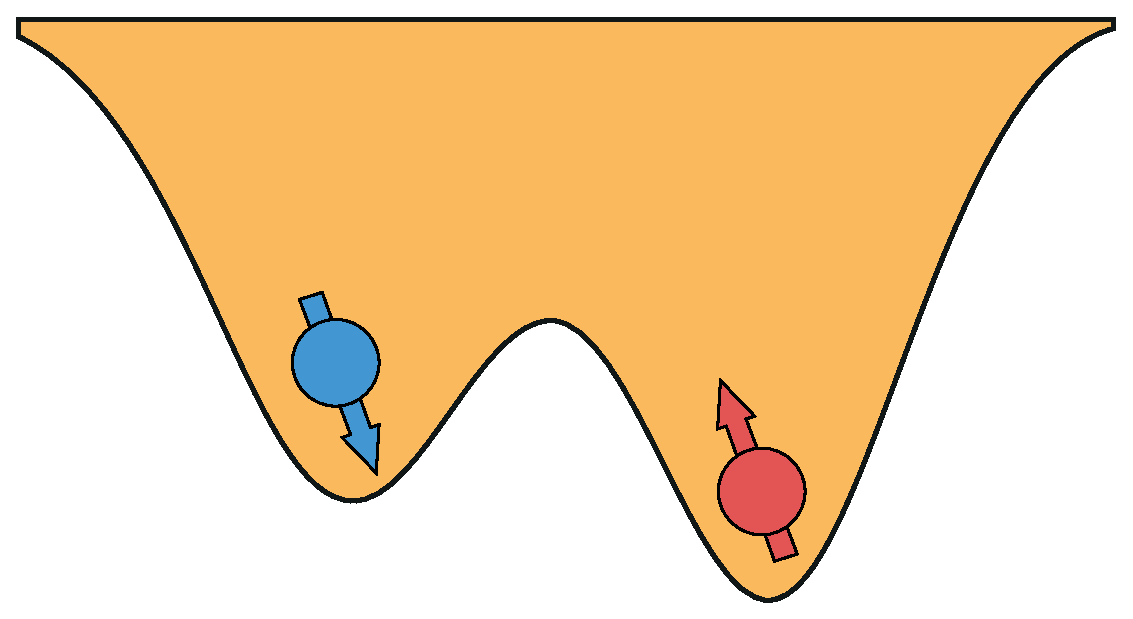
\includegraphics[width=0.6\linewidth]{cover}\\ % University/department logo - uncomment to place it

\vfill

{\scshape \textbf{Master Degree in Theoretical Physics}}\\
{\scshape Speciality in Elementary Particle Physics and Cosmology}\\% University name

 

\end{center}
\end{titlepage}


%----------------------------------------------------------------------------------------
%	ABSTRACT PAGE
%----------------------------------------------------------------------------------------

\begin{abstract}
\addchaptertocentry{\abstractname} % Add the abstract to the table of contents

\end{abstract}

%----------------------------------------------------------------------------------------
%	ACKNOWLEDGEMENTS
%----------------------------------------------------------------------------------------

\begin{acknowledgements}
\addchaptertocentry{\acknowledgementname} % Add the acknowledgements to the table of contents

\end{acknowledgements}

%----------------------------------------------------------------------------------------
%	LIST OF CONTENTS/FIGURES/TABLES PAGES
%----------------------------------------------------------------------------------------

\tableofcontents % Prints the main table of contents

%\listoffigures % Prints the list of figures

%\listoftables % Prints the list of tables

%----------------------------------------------------------------------------------------
%	ABBREVIATIONS
%----------------------------------------------------------------------------------------

\begin{abbreviations}{ll} % Include a list of abbreviations (a table of two columns)

\textbf{2DEG} & \textbf{2} \textbf{D}imensinal \textbf{E}lectron \textbf{G}as\\
\textbf{DOSS}& \textbf{D}ouble \textbf{O}ccupation \textbf{S}inglet \textbf{S}tate\\
\textbf{DQD} & \textbf{D}ouble \textbf{Q}uantum \textbf{D}ot\\
\textbf{FAQUAD} & \textbf{FA}ast \textbf{Qu}asi \textbf{A}diabatic \textbf{D}ynamics\\
\textbf{FF} & \textbf{F}ast \textbf{F}orward\\
\textbf{HH} & \textbf{H}eavy \textbf{H}ole\\
\textbf{IE} & \textbf{I}nverse \textbf{E}ngineering\\
\textbf{ODE} & \textbf{O}rdinary \textbf{D}ifferential \textbf{E}quation\\
\textbf{QD} & \textbf{Q}uantum \textbf{D}ot\\
\textbf{QPC} & \textbf{Q}uantum \textbf{P}oint \textbf{C}ontact\\
\textbf{SOC} & \textbf{S}pin-\textbf{O}rbit \textbf{C}oupling\\
\textbf{SOSS}& \textbf{S}ingle \textbf{O}ccupation \textbf{S}inglet \textbf{S}tate\\
\textbf{STA} & \textbf{S}hortcut \textbf{T}o \textbf{A}diabaticity\\
\textbf{STIRAP} & \textbf{Sti}mulated \textbf{R}aman \textbf{A}diabatic \textbf{P}assage\\
\textbf{TQD} & \textbf{T}riple \textbf{Q}uantum \textbf{D}ot


\end{abbreviations}


%----------------------------------------------------------------------------------------
%	SYMBOLS
%----------------------------------------------------------------------------------------

%\begin{symbols}{lll} % Include a list of Symbols (a three column table)
%
%$a$ & distance & \si{\meter} \\
%$P$ & power & \si{\watt} (\si{\joule\per\second}) \\
%%Symbol & Name & Unit \\
%
%\addlinespace % Gap to separate the Roman symbols from the Greek
%
%$\omega$ & angular frequency & \si{\radian} \\
%
%\end{symbols}

%----------------------------------------------------------------------------------------
%	THESIS CONTENT - CHAPTERS
%----------------------------------------------------------------------------------------

\mainmatter % Begin numeric (1,2,3...) page numbering

\renewcommand{\thechapter}{\Roman{chapter}}

\pagestyle{thesis} % Return the page headers back to the "thesis" style

% Include the chapters of the thesis as separate files from the Chapters folder
% Uncomment the lines as you write the chapters

% Chapter 1

\chapter{Introduction} % Main chapter title

\label{sec:Introduction} % For referencing the chapter elsewhere, use \ref{Chapter1} 

%----------------------------------------------------------------------------------------

% Define some commands to keep the formatting separated from the content 
\newcommand{\keyword}[1]{\textbf{#1}}
\newcommand{\tabhead}[1]{\textbf{#1}}
\newcommand{\code}[1]{\texttt{#1}}
\newcommand{\file}[1]{\texttt{\bfseries#1}}
\newcommand{\option}[1]{\texttt{\itshape#1}}

%----------------------------------------------------------------------------------------



% Chapter Template

\chapter{Quantum Dots} % Main chapter title

\label{sec:Quantum_Dots} % Change X to a consecutive number; for referencing this chapter elsewhere, use \ref{ChapterX}

%----------------------------------------------------------------------------------------
%	SECTION 1
%----------------------------------------------------------------------------------------

\section{Fundaments}

A quantum dot (QD) existentially a small ``box'' filled with particles. When the size of this region is comparable to the wavelength of the particle that populates it, the system becomes quasi 0-dimensional, exhibiting a discrete energy spectrum. This is somehow similar to an atoms, and this is why QD's are usually called artificial atoms. The dots can be filled with electrons or holes, depending on which atoms the substrate is doped with. Different sites can be coupled via tunnel barriers, allowing the particles to ``jump'' from one dot to another. It is also common to couple a source and a drain reservoir that enable the exchange of particles. By attaching current and voltage probes to these reservoirs we can measure the electronic properties of the device. This description of a QD is very general, and this is why exist systems of may different sizes and materials. For instance self-assembled quantum dots, semiconductor lateral and vertical dots, or even carbon nanotubes. An example of this devices can be found in Fig.~\ref{fig:different_devices}. In this work, we focus on lateral gated semiconductor quantum dots. These devices allow a great control over the different parameters of the system, what can be used to tune it's values in situ. 
\begin{figure}[!htbp]
	\centering
	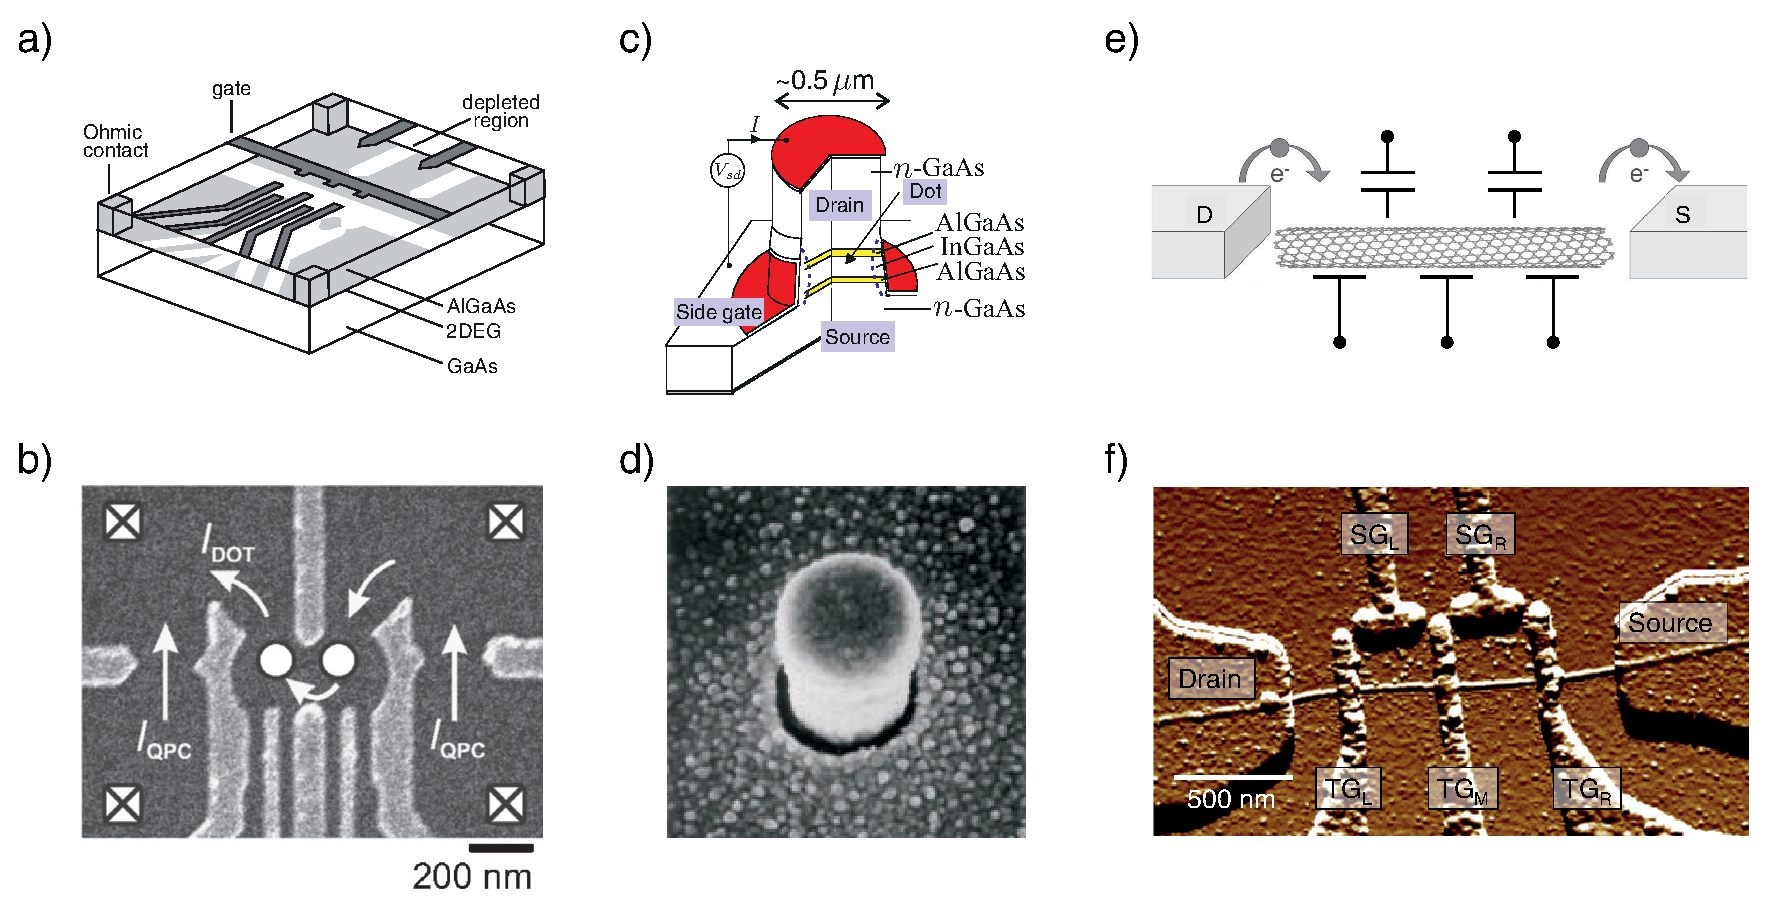
\includegraphics[width=\linewidth]{different_devices.eps}
	\caption{Different devices for quantum dots. a) Schematic view and b) scanning electron micrograph (SEM) of a lateral DQD, taken from ref. \cite{Hanson2007}. c) Schematic and d) SEM images of a vertical semiconducting QD, taken from ref. \cite{Kouwenhoven2001}. e) Schematic and f) atomic force microscope (AFM) of a DQD implemented in a carbon nanotube, taken from e) ref. \cite{SapmazPhd} and f) ref. \cite{Sapmaz2006}.}
	\label{fig:different_devices}
\end{figure}

Fabrication of gated quantum dots starts with a layered heterostructure composed by different semiconducting materials. A common choice for the semiconductors is GaAs and AlGaAs grown on top of each other. By doping the n-AlGaAs with Si we can introduce free electrons, which are accumulated in the interface forming a 2-dimensional electron gas (2DEG)\cite{Elzerman2005}. If we are interested in holes instead of electrons we can keep the GaAs/AlGaAs heterostructure undoped\cite{Tracy2014}. By applying negative voltages to metal surface electrodes (gates) on top of the semiconductor heterostructure the 2DEG is locally depleted, thereby forming the QD. In order to control the electrostatic potential of the dots with respect to the reservoirs we can couple it capacitively to a gate electrodes. The tunneling rate can be also modified with electric fields applied to the gates located between neighbouring dots. With this we have an all-electrical control over the system. We can also use a magnetic field to produce a Zeeman splitting in the spin of the particles.

\section{Transport}
The charge transport thought the system is a perfect way to measure the state of the device, since the intensity observed depends on the states of the particles inside the quantum dots. in the contacts (source and drain) there are free particles with energies up to the chemical potential $\mu$. At low temperatures this chemical potential corresponds to the Fermi energy. During the entire chapter we will consider that the temperature of the device is low enough so the approximation of the chemical potential as a step function is justified. Applying a voltage difference between the two reservoirs known as the bias voltage $V_{\text{bias}}$. The relation between this three parameters is
\begin{equation}
	V_{\text{bias}}=\frac{\mu_R-\mu_L}{e}\; ,
\end{equation}
where $L$ and $R$ denote the left and right contact respectively, and $e$ is the electron charge. The choice of the sign is a convention, different choices can be found in the literature. The chemical potential for the quantum dots is defined as the required energy to add a new particle in the site. The more particles there are in the QD, the higher is the chemical potential, thus forming what is known as the electrochemical ladder. All this discrete levels can be shifted by the gate voltage $V_G$. This is depicted in Fig.(\ref{fig:potential_ladder}). If the chemical potential of a reservoir ir larger than $\mu(N)$, then one particle can enter in the quantum dot. This will occur until the QD's potential reaches a value higher than the contact $\mu(N+1)>\mu_i$. The same thing will happen in reserve, if $\mu(N)>\mu_i$, the particles will leave the system towards the reservoir until a balance is reached. In the example shown two particles can enter initially in the QD from the right reservoir, but only one of then can tunnel out to the left drain. Then a net intensity of one particle will flow continuously from right to left.
\begin{figure}[!htbp]
	\centering
	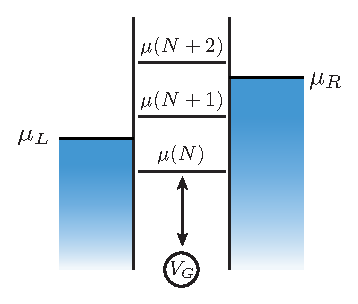
\includegraphics[width=0.4\linewidth]{potential_ladder.eps}
	\caption{Sketch of the electrochemical ladder in a quantum dot. The energy origin is given by the gate voltage $V_G$.}
	\label{fig:potential_ladder}
\end{figure}

In order to know exactly the number of particles inside the devices we must use the stability diagrams. This kind of measures can be obtained by two different techniques, but with very similar results. In both of them the chemical potential of the reservoirs are keep constant and equal to each other, that is $V_{\text{bias}}=0$. Then the gate voltages of each dot are modified independently, trying to map out as much of the area as possible. The aim of these measures is to obtain at which values fir the gate voltages there is a variation in the number of particles. One possibility for this is the use of a quantum point contact (QPC), which is sensitive to the variation of charge inside the QD. On the other hand, we can determine this movement of the particles also via the charge intensity. Both methods assume a sequential tunneling, that is, only one particle enter or exit the device at each time, so every time a transition is measured, either with the QCP or with the electronic intensity, we can assure that only one particle has changed its position. Once we don't see any more transitions all the QD's are empty, allowing us to define the exact number of particles for each quantum dot in each region.

\subsection{Coulomb Blockade}

\subsection{Pauli Blockade}

\section{Quantum Gates with QD}

 
% Chapter Template

\chapter{Shortcuts to Adiabaticity and Robustness} % Main chapter title

\label{sec:Shortcuts_to_Adiabaticity} % Change X to a consecutive number; for referencing this chapter elsewhere, use \ref{ChapterX}

%----------------------------------------------------------------------------------------
%	SECTION 1
%----------------------------------------------------------------------------------------

The manipulation of a quantum system has important consequences in quantum computation, since with this we are able to initialize the qubits and perform different quantum gates. One possibility to obtain high fidelities is to prepare the system in the ground state and then adiabatically transfer the state to the target state by modification the Hamiltonian. One example of this is the coherent transfer by adiabatic passage (CTAP) \cite{Greentree2004}. One popular option is the use of Gaussian pulses to realize the adiabatic transfer
\begin{equation}
	\lambda_i(t)=\lambda_i^{\max}\exp[-(t-t_i)^2/(2\sigma_i^2)]\; ,
\end{equation}
where $\lambda_i(t)$ represents all the possible time dependent parameters in the system. In order to prevent the excited states leakages at the avoided crossings the change in the Hamiltonian must be infinitesimal, meaning that the manipulation total time tends to infinity. For practical applications this is neither possible nor desirable as we want protocols capable of implementing operations in the qubits as fast as possible. In addition, there is one more problem when working with such long times, and that is that the dephase and decoherence accumulate over time, causing us to move out of the desired state and thus obtaining low fidelities. During the last decade there has been a great proliferation of so calls Shortcut to Adiabaticity (STA) \cite{Chen2010}, which aim not only to speed up the protocols but also to increase the robustness against possible experimental errors. Since adiabatic passages are a widespread method for the manipulation of a system, many different protocols can be classified under the name STA. Each different approach has its own features, some get analytical results while others must be solved numerically, some are focused on minimizing operating time, whereas other have as their main task to obtain the lowest possible sensitivity to noise. This is why a study must first be made to choose the most appropriate technique in each case. Here we will present a summary of the most used techniques, presenting their main advantages and disadvantages.

\section{\label{sec:CD}Counteradiabatic driving}
The basic idea of counteradiabatic driving (CD), also known as transitionless quantum driving, is the addition of a new term to the original Hamiltonian $H_0(t)$ so that the dynamic of the state follow exactly the adiabatic evolution. This can be seen as a classical system to which we apply an external force in order the dynamic follows a certain trajectory. There exist two equivalent theoretical approaches for this STA protocol, the formulation of Demirplak and Rice \cite{Demirplak2003}, and the Berry's formulation \cite{Berry2009}. This last one is the one we will see here. Let's start with the original Hamiltonian, which can be written in a general form as
\begin{equation}
	\hat{\mathcal{H}}_0(t)=E_n(t)\sum_n\ket{\phi_n(t)}\bra{\phi_n(t)}\; ,
\end{equation}
with $\ket{\phi_n(t)}$ the instant eigenvectors and $E_n(t)$ the corresponding energies. Let the system start at a given instant state $\ket{\phi_n(0)}$, if the driving is slow enough the system will continue in the same state up to a phase
\begin{equation}
	\ket{\psi_n(t)}=e^{i\xi_n(t)}\ket{\phi_n(t)}\;.
\end{equation}
This phase that the state acquire can be obtained by substituting the above ansatz in the time dependent Schrödinger equation $i\hbar\partial_t\ket{\psi_n(t)}=H_0(t)\ket{\psi_n(t)}$, resulting in
\begin{equation}
	i\hbar\left(i\partial_t\xi_n(t)e^{i\xi_n(t)}\ket{\phi_n(t)}+e^{i\xi_n(t)}\partial_t\ket{\phi_n(t)}\right)=E_n(t)e^{i\xi_n(t)}\ket{\phi_n(t)}\; .
\end{equation}
Simplifying the phase factors and using the orthonormality of the states at any time $\braket{\phi_n(t)}{\phi_{n'}(t)}=\delta_{nn'}$ we obtain the result
\begin{equation}
	\xi_n(t)=-\frac{1}{\hbar}\int_0^tdt'E_n(t')+i\int_0^tdt'\braket{\phi_n(t')}{\partial_t \phi_n(t')}\; .
	\label{eq:Berry_phase}
\end{equation}
The first term is the typical phase acquired due to the state time evolution and the second term in known as the Berry phase, also known as the geometric phase. We are searching for a time evolution that follows the adiabatic states regardless the speed of the protocol, so the unitary evolution operator is
\begin{equation}
	U(t)=\sum_n\ket{\psi_n(t)}\bra{\psi_n(0)}=\sum_ne^{i\xi_n(t)}\ket{\phi_n(t)}\bra{\phi_n(0)}\; .
\end{equation}
Using this operator we can compute the Hamiltonian needed using $\hat{\mathcal{H}}(t)=i\hbar \dot{U}U^\dag$,  where the dot means the time derivative. Substituting the operator that we have just obtained we have
\begin{equation}
	\begin{split}
	\hat{\mathcal{H}}(t)&=i\hbar\left(\sum_ni\dot{\xi_n}(t)e^{i\xi_n(t)}\ket{\phi_n(t)}\bra{\phi_n(0)}+e^{i\xi_n(t)}|\dot{\phi}_n(t)\rangle\bra{\phi_n(0)}\right)\\
	&\phantom{=i\hbar}\times\left(\sum_{n'}e^{-i\xi_{n'}(t)}\ket{\phi_{n'}(0)}\bra{\phi_{n'}(t)}\right)\\
	&=i\hbar\sum_ne^{i\xi_n(t)}\left[i\left(-\frac{1}{\hbar}E_n(t)+i\bra{\phi_n(t)}\dot{\phi}_n(t)\rangle\right)\ket{\phi_n(t)}+|\dot{\phi}_n(t)\rangle\right]\\
	&\phantom{=i\hbar}\times\sum_{n'}e^{-i\xi_{n'}(t)}\delta_{nn'}\bra{\phi_{n'}(t)}\\
	&=\sum_nE_n(t)\ket{\phi_n(t)}\bra{\phi_n(t)}+i\hbar\sum_n\left(|\dot{\phi}_n(t)\rangle\bra{\phi_n(t)}-\bra{\phi_n(t)}\dot{\phi}_n(t)\rangle\ket{\phi_n(t)}\bra{\phi_n(t)}\right)\; ,
	\end{split}
\end{equation}
where the first term in the last line corresponds to the original Hamiltonian and the second term is the new counterterm Hamiltonian that we must add $\hat{\mathcal{H}}(t)=\hat{\mathcal{H}}_0(t)+\hat{\mathcal{H}}_{\text{CD}}(t)$ to ensure that the initial state follows the adiabatic path.\\

With this scheme we have a great deal of freedom to choose the evolution of the parameters, the simplest choice is a polynomial interpolation fulfilling the boundary conditions given by the initial and final target states. However, in order the use CD we must know all the eigenstates of the system, what can be really difficult in many body systems, this is one of the main disadvantages of the scheme. It may also be the case that the counterterm Hamiltonian include term which are in principle not controllable and in general not possible to produce in a given experimental setup. Lot of effort is being put into solving these kind of problems \cite{Ibanez2011,Chen2017,Petiziol2018,Baksic2016}.

\section{FAQUAD}
Let $\ket{\phi_1(t)}$ and $\ket{\phi_2(t)}$ the instant basis for a two level system with energies $E_1$ and $E_2$ respectively. Initialising the system in one of these states, $\ket{\phi_1}$ for instance, the evolution will maintain in this instant state, up to a phase, if the adiabatic condition is fulfilled \cite{Schiff1968}
\begin{equation}
	\hbar\abs{\frac{\braket{\phi_1(t)}{\partial_t\phi_2(t)}}{E_1(t)-E_2(t)}}=c\ll 1\;.
	\label{eq:adiabatic_condition}
\end{equation}
In order to simplify the numerator we can start with the time independent Schrödinger equation which defines the instant eigenstate $\ket{\phi_2(t)}$. If we derivate the expression and multiply by $\bra{\phi_1(t)}$ we can obtain
\begin{equation}
	\begin{split}
	\hat{\mathcal{H}}\ket{\phi_2}&=E_2\ket{\phi_2}\\
	(\partial_t \hat{\mathcal{H}})\ket{\phi_2}+\hat{\mathcal{H}}\ket{\partial_t\phi_2}&=(\partial_t E_2)\ket{\phi_2}+E_2\ket{\partial_t\phi_2}\\
	\bra{\phi_1}\partial_t \hat{\mathcal{H}}\ket{\phi_2}+\bra{\phi_1}\hat{\mathcal{H}}\ket{\partial_t \phi_2}&=(\partial_t E_2)\braket{\phi_1}{\phi_2}+E_2\braket{\phi_1}{\partial_t \phi_2}\\
	\bra{\phi_1}\partial_t \hat{\mathcal{H}}\ket{\phi_2}+E_1\braket{\phi_1}{\partial_t\phi_2}&=E_2\braket{\phi_1}{\partial_t\phi_2}\\
	\braket{\phi_1}{\partial_t \phi_2}&=\frac{\bra{\phi_1}\partial \hat{\mathcal{H}}\ket{\phi_2}}{E_2-E_1}\; .
	\end{split}
\end{equation}
In the third step we have used the orthogonality if the adiabatic states $\braket{\phi_i}{\phi_j}=\delta_{ij}$. So the Hamiltonian $H(t)$, the instant energies $E_i(t)$ and the adiabatic states $\phi_i(t)$ depend on the time, in order to obtain nicer expressions in the above equation we have relaxed the notation by dropping off all the explicit dependences of time. Using this result in Eq.~(\ref{eq:adiabatic_condition}) we obtain a reformulated adiabatic condition
\begin{equation}
	\hbar\abs{\frac{\bra{\phi_1(t)}\partial_t \hat{\mathcal{H}}(t)\ket{\phi_2(t)}}{\left[E_1(t)-E_2(t)\right]^2}}=c\ll 1\; .
\end{equation}
This was the case of a two level system, the extension for a multi-level system is straightforward
\begin{equation}
	\hbar\sum_{n\neq i}\abs{\frac{\bra{\phi_i(t)}\partial_t \hat{\mathcal{H}}(t)\ket{\phi_n(t)}}{\left[E_i(t)-E_n(t)\right]^2}}=c\ll 1\; ,
	\label{eq:multilevel_adiabatic_condition}
\end{equation}
where the index $i$ denotes the state in which we initialize the system. Looking at this equation we observe that the larger the gap between energies the faster we can go from the initial to the final state maintaining the adiabatic condition. If the gap is too tight the evolution must be slow enough so the dynamics follow the adiabatic states. This is the heart of the fast quasi-adiabatic (FAQUAD) protocol \cite{MartinezGaraot2015}, when the states are far away in energies the protocol can be as fast as possible, but it must slow down when we are approaching to a avoided crossing in which the energies are close to each other. In a simple scenario we can assume that the adiabatic process is driven by just one parameter $\lambda(t)$. Using the chain rule we can write $\partial_t=\partial_\lambda \dot{\lambda}$ and substituting in Eq.~(\ref{eq:multilevel_adiabatic_condition}) we can obtain the variation of the parameters
\begin{equation}
	\dot{\lambda}=\pm \frac{c}{\hbar}\left(\sum_{n\neq i}\abs{\frac{\bra{\phi_i(\lambda)}\partial_\lambda \hat{\mathcal{H}}(\lambda)\ket{\phi_n(\lambda)}}{\left[E_i(\lambda)-E_n(\lambda)\right]^2}}\right)^{-1}\; ,
	\label{eq:parameter_ODE}
\end{equation}
where the sign $\pm$ correspond to a monotonous increase/decrease of the parameter. It is usual to work with the rescaled time $s\equiv t/t_f$ and redefine the adiabatic parameter as $\tilde{c}\equiv ct_f$ with $t_f$ the total time of the protocol. Setting $\tilde{c}$ constant over all times we can obtain its value computing the following integral which is easily derivate from Eq.~(\ref{eq:parameter_ODE})
\begin{equation}
	\int_0^1 ds\tilde{c}=\tilde{c}=\int_{\lambda(t=0)}^{\lambda(t=t_f)}d\lambda \left(\sum_{n\neq i}\abs{\frac{\bra{\phi_i(\lambda)}\partial_\lambda \hat{\mathcal{H}}(\lambda)\ket{\phi_n(\lambda)}}{\left[E_i(\lambda)-E_n(\lambda)\right]^2}}\right)\; ,
	\label{eq:c_tilde_deff}
\end{equation}
what can be done analytically or numerically. Here we can see that $\tilde{c}$ is independent of the final time, what means that the adiabatic parameter $c\propto 1/t_f$. This is something we have predicted, the longer the protocol, the more adiabatic the process. Let us introduce a new notation for the parameter in terms of the rescaled time $\tilde{\lambda}(s)\equiv \lambda(s t_f)$ and it's derivative denote by $\tilde{\lambda}'(s)\equiv t_f\dot{\lambda}(t)$. With this new convention we can rewrite Eq.~(\ref{eq:parameter_ODE}) as
\begin{equation}
\tilde{\lambda}'(s)=\pm \frac{\tilde{c}}{\hbar}\left(\sum_{n\neq i}\abs{\frac{\bra{\phi_i(\tilde{\lambda})}\partial_{\tilde{\lambda}} \hat{\mathcal{H}}(\tilde{\lambda})\ket{\phi_n(\tilde{\lambda})}}{\left[E_i(\tilde{\lambda})-E_n(\tilde{\lambda})\right]^2}}\right)^{-1}\; .
\label{eq:parameter_ODE_2}
\end{equation}
Once we compute the value for $\tilde{c}$, we can numerically solve the above ordinal differential equation (ODE) an obtain the evolution for the parameter $\tilde{\lambda}(s)$. If the adiabatic condition is verified $\tilde{c}/t_f\ll 1$ then the wave function that describes the system can be expanded using adiabatic perturbation theory as
\begin{equation}
	\ket{\Psi(t)}=\sum_na_n(t)e^{i\xi_n(t)}\ket{\phi_n(t)}\; ,
	\label{eq:adiabatic_approx_1}
\end{equation}
where we phase is exactly the same than the one described in Eq.~(\ref{eq:Berry_phase}). Introducing Eq.~(\ref{eq:adiabatic_approx_1}) in the time dependent Schrödinger equation we obtain a system of ODEs for the amplitude of each instant eigenvector
\begin{equation}
	\begin{split}
	i\hbar\left[\sum_k\dot{a}_k(t)e^{i\xi_k(t)}\ket{\phi_k(t)}+ia_k(t)\dot{\xi}_k(t)e^{i\xi_k(t)}\ket{\phi_k(t)}\right.&\\
	\left.+a_k(t)e^{i\xi_k(t)}|\dot{\phi}_k(t)\rangle\right]&=\sum_k a_k(t)e^{i\xi_k(t)E_k\ket{\phi_k(t)}}
	\end{split}
\end{equation}
what can be easily simplified to the expression
\begin{equation}
	\sum_k \dot{a}_k(t)e^{i\xi_k(t)}\ket{\phi_k(t)}=-\sum_ka_k(t)e^{i\xi_k(t)}|\dot{\phi}_k(t)\rangle\; .
\end{equation}
Multiplying both sides of the equation by $\ket{\phi_n(t)}$ with $n\neq k$, and imposing $\bra{\phi_k}\dot{\phi}_k(t)\rangle=0$ we obtain the equation
\begin{equation}
	\dot{a}_n(t)=-\sum_{k\neq n}a_k(t)e^{iW_{nk}(t)}\bra{\phi_n(t)}\dot{\phi}_k(t)\rangle\; ,
	\label{eq:EDO_coefficient}
\end{equation}
where we have defined the phase $W_{nk}\equiv \int_0^t\omega_{nk}(t')dt$ with
\begin{equation}
	\omega_{nk}(t)\equiv \frac{1}{\hbar}[E_n(t)-E_k(t)]\; .
\end{equation}
Integrating Eq.~(\ref{eq:EDO_coefficient}) we have
\begin{equation}
	a_n(t)-a_n(0)=-\sum_{k\neq n}\int_0^te^{iW_{nk}(t')}\bra{\phi_n(t')}\dot{\phi}_k(t')\rangle a_k(t') dt'\; .
\end{equation}
We initialise the system in one of the instant states $\ket{\Psi(t=0)}=\ket{\phi_i(t=0)}$, so at first order in adiabatic perturbation theory we can set $a_k(t')=\delta_{ki}$. Using this in the above equation we obtain
\begin{equation}
	a_n^{(1)}(t)=-\int_0^te^{iW_{ni}(t')}\bra{\phi_n(t')}\dot{\phi}_i(t')\rangle dt'\; ,
	\label{eq:almost_done}
\end{equation}
which should satisfy $\abs{a_n^{(1)}(t)}\ll 1$ for an adiabatic evolution. We can compute this integral for FAQUAD using Eq.~(\ref{eq:multilevel_adiabatic_condition}) we can write
\begin{equation}
	\bra{\phi_n(t)}\dot{\phi}(t)_i\rangle=c_nr\omega_{ni}(t)\; .
\end{equation}
with $r\equiv\operatorname{sgn}[\bra{\phi_n(t)}\dot{\phi}_i(t)\omega_{ni}]$ and $c=\sum_{n\neq i}c_n$. Using this in Eq.~(\ref{eq:almost_done}) we obtain the final result of
\begin{equation}
	a_n^{(1)}(t)=-c_nr\int_0^t\omega_{ni}(t')e^{iW_{ni}(t')}dt'=ic_nr\left(e^{iW_{ni}(t)}-1\right)\; .
\end{equation}
With this we can compute the population of the $n$-state at first order as
\begin{equation}
	\abs{\braket{\phi_n(t)}{\Psi(t)}}^2=\abs{a^{(1)}_n(t)}^2=2c_n^2\left[1-\cos(W_{ni}(t))\right]\; .
	\label{eq:amplitudes_adiabatic}
\end{equation}
The upper limit for the state is given by
\begin{equation}
	\abs{a_n^{(1)}(t)}^2\leq 4c^2\; .
\end{equation}
Defining the fidelity as the probability of measuring the initial eigenvector at the final time $\mathcal{F}\equiv \abs{\braket{\phi_i(t=t_f)}{\Psi(t=t_f)}}^2$, we can use Eq.~(\ref{eq:amplitudes_adiabatic}) to obtain the expression
\begin{equation}
	\mathcal{F}^{(1)}=1-\sum_{n\neq i}\abs{a_n^{(1)}(t_f)}^2=1-2\sum_{n\neq i}c_n^2\left[1-\cos(W_{ni}(t_f))\right]\; .
	\label{eq:FAQUAD_fidelity}
\end{equation}
With this we can extract that in a system with $N$ levels, the fidelity, in terms of the final time, presents an oscillatory behaviour governed by $N-1$ frequencies given by the equation
\begin{equation}
	\nu_{ni}=\frac{1}{2\pi\hbar}\int_0^1\abs{E_n(s)-E_i(s)}ds\; .
	\label{eq:FAQUAD_frecuencies}
\end{equation}
Using Eq.~(\ref{eq:FAQUAD_fidelity}) we predict a lower bound for the fidelity in terms of the final time
\begin{equation}
	\mathcal{F}^{(1)}\geq 1-4\sum_{n\neq i}c_n^2=1-\frac{4}{t_f^2}\sum_{n\neq i}\tilde{c}_n^2\; .
	\label{eq:lower_bound_fidelity}
\end{equation}

One of the strengths of FAQUAD is that we can compute the evolution of the parameter $\lambda(t)$ without the need of a analytical solution for the eigenstates and eigenenergies of the system. This is really important if we want to use this method in a multi-level Hamiltonian whose structure is difficult enough to solve the equations analytically. One more advantage is that we have not included additional terms to the Hamiltonian, in contrast to what we have seen with the CD approach. Solving Eq.~(\ref{eq:parameter_ODE_2}) we compute the driving parameter $\tilde{\lambda}(s)$ in terms of the scaled time $s$, without specifying a value for $t_f$. The equation only needs to be solve once and can be used for any total time, saving time of computation. One of the main weaknesses of FAQUAD is that, like CD, total system information (eigenstates and eigenvectors) is needed, what may be difficult for many body systems. To alleviate this we can used the local adiabatic approach \cite{Roland2002}, which change Eq.~(\ref{eq:parameter_ODE_2}) in favour of
\begin{equation}
\tilde{\lambda}'(s)=\pm \frac{\tilde{c}}{\hbar}\left(\sum_{n\neq i}\abs{\frac{\partial_{\tilde{\lambda}}[E_i(\tilde{\lambda})-E_n(\tilde{\lambda})]} {\left[E_i(\tilde{\lambda})-E_n(\tilde{\lambda})\right]^2}}\right)^{-1}\; ,
\end{equation}
that only needs the eigenenergies of the system, reducing drastically the amount of information needed. However, as one would expect, the results obtained produce lower fidelity than when using FAQUAD.

\section{Inverse engineering}
The last STA scheme that we will comment here is inverse engineering \cite{Chen2012}. This protocol is quite simple in its basis but has a huge flexibility. The main idea is to parametrize the solution of the wave function, and them solve the time-dependent Schrödinger equation to obtain the differential equations that these parameters, also called auxiliary parameters, that we have added must verify. This system of ODEs can be inverted to obtain the time dependent function for the parameters of the system, also known as controlling parameters, those that are in the Hamiltonian. Lastly we made some ansatz for the auxiliary parameters that verify the required boundary conditions to perform the desired transfer. More boundary conditions can be imposed to the derivatives of the auxiliary parameters in order to obtain smooth and well-behaviour pulses. Thanks to this freedom in the choice of the interpolated function we can design protocols optimized to has low sensitivity in possible errors, or protocols whose aim is to speed up the transfer to diminish the effect of coherence and relaxing times.

The potential of this protocol lies in the choice of a good parametrization, what can be a quit difficult task. This is why it's usual to combine this scheme with other protocols as the Lewis-Riesenfeld invariants \cite{Lewis1969}. 

\section{Robustness}
The existence of errors in the devices and the appearance of noise in these is something difficult to deal with when conducting the experiments, so it is important to take it into account when running the numerical simulations. These sources of error that lead to lower fidelity can be grouped into two main categories known as systematic errors and stochastic errors. The first one correspond to a bad calibration of the devices yielding values for the system parameters that systematically deviate from those imposed by the STA schemes. Letting $\hat{\mathcal{H}}_0(t)$ be the ideal Hamiltonian, this systematic effects can be taken into account by adding a new term to the total Hamiltonian
\begin{equation}
	\hat{\mathcal{H}}_T(t)=\hat{\mathcal{H}}_0(t)+\delta_0\hat{\mathcal{H}}_1(t)\; ,
\end{equation}
where $\hat{\mathcal{H}}_1(t)$ is the part of the original Hamiltonian contributing from the parameter in which we are interested. The other possible source of error is the existence of noise in the experimental step-up what can be simulated with the Schrödinger equation that depends on a white noise $\zeta(t)$ and the parameters that suffer from the noise included in $\hat{\mathcal{H}}_2$. In the Stratonovich sense this stochastic equation is written as
\begin{equation}
	i\hbar \partial_t\ket{\Psi(t)}=(\hat{\mathcal{H}}_0(t)+\gamma_0\hat{\mathcal{H}}_2(t)\zeta(t))\ket{\Psi(t)}\; .
\end{equation}
The function $\zeta(t)$ is the derivative of a Brownian motion, and the conditions that must fulfil to represent a white noise is to have zero mean value $\expval{\zeta(t)}=0$ and the values at different times must be uncorrelated $\expval{\zeta(t)\zeta(t')}=\delta(t-t')$. The dynamical equation for the stochastic density matrix can be obtained from the above equation as
\begin{equation}
	\frac{d}{dt}\rho_\zeta=-\frac{i}{\hbar}[\hat{\mathcal{H}}_0(t),\rho_\zeta]-\frac{i\gamma_0}{\hbar}[\hat{\mathcal{H}}_2(t),\zeta\rho_\zeta]\; .
	\label{eq:stochastic_dynamics}
\end{equation}
Averaging over different realizations the equation is written as
\begin{equation}
	\frac{d}{dt}\rho=-\frac{i}{\hbar}[\hat{\mathcal{H}}_0(t),\rho]-\frac{i\gamma_0}{\hbar}[\hat{\mathcal{H}}_2(t),\expval{\zeta\rho_\zeta}]\; ,
	\label{eq:almost_dynamic_eq}
\end{equation}
where we have defined the mean density matrix as $\rho(t)=\expval{\rho_\zeta(t)}$. In order to simplify the expected value we can use the Navikov's theorem which reads
\begin{equation}
	\expval{\zeta(t)\mathscr{F}[\zeta(t)]}=\int_0^tds\expval{\zeta(t)\zeta(s)}\expval{\frac{\partial\mathscr{F}[\zeta]}{\partial\zeta(s)}}
\end{equation}
with $\mathscr{F}[\zeta(t)]$ some function that depends on the noise. Using the fact that we are dealing with a white noise the above equation is simplified as\footnote{Recall that in the Stratonovich interpretation $\int_0^\infty dt\delta (t)=1/2$.}
\begin{equation}
	\expval{\zeta(t)\mathscr{F}[\zeta(t)]}=\frac{1}{2}\expval{\frac{\partial\mathscr{F}[\zeta]}{\partial \zeta(s)}}_{s=t}\; .
	\label{eq:Navikovs_result}
\end{equation}
Integrating Eq.~(\ref{eq:stochastic_dynamics}) we obtain the expression
\begin{equation}
	\rho_\zeta=-\frac{i}{\hbar}\int_0^tds[\hat{\mathcal{H}}_0(s),\rho_\zeta(s)]-\frac{i\gamma_0}{\hbar}\int_0^tds[\hat{\mathcal{H}}_2(s),\rho_\zeta(s)]\zeta(s)\; ,
\end{equation}
and with the substitution $\mathscr{F}[\zeta(t)]=\rho_\zeta(t)$ and using this above integral in Eq.~(\ref{eq:Navikovs_result}) we have
\begin{equation}
	\expval{\zeta\rho_\zeta}=-\frac{i\gamma_0}{2\hbar}[\hat{\mathcal{H}}_2(t),\rho(t)]\; .
\end{equation}
Inserting this result in Eq.~(\ref{eq:almost_dynamic_eq}) we obtain finally the matrix differential equation that governs the dynamics of the density matrix under a stochastic white noise
\begin{equation}
	\frac{d}{dt}\rho=-\frac{i}{\hbar}[\hat{\mathcal{H}}_0(t),\rho]-\frac{\gamma_0^2}{2\hbar^2}[\hat{\mathcal{H}}_2(t),[\hat{\mathcal{H}}_2(t),\rho]]\; .
\end{equation}
This expression is reminiscent of Lindblad's master equation, with the difference that here we are taking into account amplitude-noise effects and not decoherence and relaxation. The Lindblad equation, also known as the Lindbladian, is written in the diagonal form as
\begin{equation}
	\frac{d}{dt}\rho=-\frac{i}{\hbar}[\hat{\mathcal{H}}(t),\rho]+\sum_{i}\gamma_i\left(\mathcal{L}_i\rho\mathcal{L}^\dagger_i-\frac{1}{2}\left\{\mathcal{L}_i^\dagger\mathcal{L}_i,\rho\right\}\right)\; ,
	\label{eq:Lindblad_ME}
\end{equation}
where $\mathcal{L}_i$ are called the Lindblad operators or collapse operators. Here we have written the general equation in which more than one different operators can be present in the system. This operators represent the how the environment couples to the system with the corresponding rates $\gamma_i$. One possibility is the study of pure dephasing contributions, which leads to the master equation
\begin{equation}
	\frac{d}{dt}\rho=-\frac{i}{\hbar}[\hat{\mathcal{H}}(t),\rho]-\frac{\gamma}{2}(\rho-\operatorname{diag}(\rho))\; .
	\label{eq:dephasing_ME}
\end{equation}
This equation can be written in term of the generalized Pauli matrices of higher dimension, beings $\sigma_{ii}^d$ the diagonal matrices of dimension $d$. The above equation can be written setting $\mathcal{L}_i=\sigma_{ii}$ and $\gamma_{i}=\gamma$ in Eq.~(\ref{eq:Lindblad_ME}). The construction of these diagonal matrices can be easily achieved as
\begin{equation}
	\sigma_{ii}^d=\left\{\begin{array}{lr}
	\mathds{1}_d & \text{for } k=1\\
	\sigma_{ii}^{d-1}\oplus 0 & \text{for } 1<i<d\\
	\sqrt{\frac{2}{d(d-1)}}(\mathds{1}_{d-1}\oplus (1-d)) &\text{for } i=d
	\end{array}\right. \; .
	\label{eq:diagonal_matrices}
\end{equation}
where $\mathds{1}_d$ denotes the identity matrix of dimension $d$, and $\oplus$ means the matrix direct sum. Setting $d=2$ we have the well known Pauli matrix
\begin{equation}
	\sigma_{11}^2\equiv \sigma_z=\mqty(1 & 0 \\ 0 & -1)\; .
\end{equation}
Increasing the dimension by one, i.e. $d=3$, we have the two diagonal Gell-Mann matrices
\begin{equation}
	\sigma_{11}^3\equiv \lambda_3=\mqty(1 & 0 & 0 \\ 0 & -1 & 0 \\ 0 & 0 & 0), \quad \sigma_{22}^3\equiv \lambda_8=\frac{1}{\sqrt{3}}\mqty(1 & 0 & 0 \\ 0 & 1 & 0 \\ 0 & 0 & -2)\;.
\end{equation}
With this procedure we can obtain the matrices $\sigma_{ii}^d$ with any dimension. As  is obvious, the value of $d$ must correspond to the number of states in our Hamiltonian.\\


At some points of this work we will mention the sensitivity of the protocol to variations of some parameter. Let us denote with $\lambda$ some parameter in which we are interested, we define the sensitivity of the fidelity to changes in this parameter as the derivative $\partial \mathcal{F}/\partial \lambda$. This corresponds to the intuitive idea that if the fidelity presents abrupt variations the sensitivity is high, while if the fidelity has presents a constant value the protocol is insensitive to changes in the parameter.






% Chapter Template

\chapter{Theoretical Model for QD's} % Main chapter title

\label{sec:Model} % Change X to a consecutive number; for referencing this chapter elsewhere, use \ref{ChapterX}

%----------------------------------------------------------------------------------------
%	SECTION 1
%----------------------------------------------------------------------------------------

The hole manifold is composed of two heavy holes (HH) and two light holes (LH), with $J_Z=\pm3/2$ and $J_Z=\pm1/2$ respectively. The kinetic term for both particles in bulk can be described with the Luttinger-Kohn Hamiltonian \cite{Bulaev2005,Luttinger1956} as
\begin{equation}
	\hat{T}_{\text{HH}(LH)}=\frac{\gamma_1\pm \gamma_2}{2m_0}(p_x^2+p_y^2)+\frac{\gamma_1\mp 2\gamma_2}{2m_0}p_z^2+U(x,y)+V_H(z)\; ,
\end{equation}
where $p_i$ are the usual momentum operators, $m_0$ the free electron mass, $U(x,y)$ the lateral confinement produced by the gates and $V_H(z)$ the vertical confinement produced by the interphase in the heterostructure. The effective mass depends on the Luttinger parameters, corresponding to $\gamma_1=6.95$  and $\gamma_2=2.25$ in GaAs \cite{Bogan2018}, obtaining the masses $m_{\text{HH}}(z)=0.41m_0$ and $m_{\text{LH}}(z)=0.09m_0$. If the vertical confinement, parallel to the [001] growth direction, is strong enough the hole subband split, with the HH subband lying lower in energies than the LH subband, and the mixing between them are much smaller than the other parameters of the system. This allows us to work with the perturbative Hamiltonian for a single confined HH as
\begin{equation}
	\hat{\mathcal{H}}_0=\frac{1}{2m}(p_x^2+p_y^2)+U(x,y)\; .
\end{equation}
with $m$ the effective HH mass. We must also take into account the spin-orbit coupling (SOC) given by the Hamiltonian
\begin{equation}
	\hat{\mathcal{H}}_{SO}=-\beta (\sigma_+p_-p_+p_-+\sigma_-p_+p_-p_+) + iE_\perp\alpha(\sigma_+p_-^3-\sigma_-p_+^3)\; .
	\label{eq:SOC_Hamiltonain}
\end{equation}
here we have defined the operators $p_\pm=p_x\pm ip_y$ and the combination of Pauli matrices $\sigma_{\pm}=(\sigma_x\pm i\sigma_y)/2$. The parameter $E_\perp$ denotes the effective electric field produced by the accumulation gate, and the momentum operator $\vec{p}=-i\hbar\vec{\nabla}+\frac{e^*}{c}\vec{A}$ contains the magnetic-field potential dependence with $e^*$ being the effective hole electric charge and $c$ the speed of light. The SOC consists in two different contributions: the Dresselhaus term ($\beta$) due to the bulk inversion asymmetry \cite{Dresselhaus1955} and the Rashba spin-orbit ($\alpha$) due to the structure inversion asymmetry \cite{Bychkov1984}. The coupling between HH and LH also produce a new SOC term\cite{Bulaev2007}, but it's value is much smaller that the two here commented, so we will not include it in our model. We are interested in a phenomenological model, so we can rewrite the above Hamiltonians using a simple Hubbard-Anderson \cite{1963a,Anderson1961,Traa1994} model consisting of $N$ impurities. The total Hamiltonian can be summarized as
\begin{equation}
	\hat{\mathcal{H}}=\hat{\mathcal{H}}_{\text{QD}}+\hat{\mathcal{H}}_B+\hat{\mathcal{H}}_{\text{SO}}\; ,
	\label{eq:total_Hamiltonian}
\end{equation}
with the first term representing the array of quantum dots
\begin{equation}
	\hat{\mathcal{H}}_{\text{QD}}=\sum_{i=1}^N\varepsilon_{i}\hat{c}^\dagger_i\hat{c}_i+\sum_{i=1}^NU_i\hat{n}_{i\uparrow}\hat{n}_{i\downarrow}+\sum_{i\neq j}\frac{U_{ij}'}{2}\hat{n}_i\hat{n}_j-\sum_{i\neq j,\sigma}t_{N,ij}(\hat{c}^\dagger_{i\sigma}\hat{c}_{j\sigma}+ \text{H.c.})\; .
\end{equation}
The first term on the right hand side ot the above equation represents the on-site energy $\varepsilon_{i}$ of the dot $i$, the second and third terms are the intradot $U_i$ and interdot $U_{ij}'$ Coulomb interactions respectively, which can depend on the sites. Finally the fourth term corresponds to the spin-conserving tunneling rate $t_{N,ij}$ between dots $i$ and $j$. The annihilation (creation) fermionic operators on the site $i$ and with spin $\sigma=\uparrow,\downarrow$ are given by $\hat{c}^{i\sigma}$ ($\hat{c}_{i\sigma}^\dagger$), and $\hat{n}_{i\sigma}$ is the particle number operator. To keep the computations as simpler as possible it is common to neglect the interdot Coulomb interactions, so we set $U_{ij}'=0$. In the above Hamiltonian we have only considered the ground state of each orbital, neglecting excited states. This is justified if the relevant energies are $\ll U_i$, what we will see in next section that is our case. In this work we will treat with linear arrays of QD in the approximation of first neighbour coupling, so tunneling will be only available for adjacent dots. The second term of Eq.~(\ref{eq:total_Hamiltonian}) represents the Zeeman splitting due to a magnetic filed perpendicular to the QD's plane
\begin{equation}
	\hat{\mathcal{H}}_{\text{B}}=\frac{1}{2}g^*\mu_B B_\perp\sum_{i=1}^N(\hat{n}_{i\uparrow}-\hat{n}_{i\downarrow})\; ,
\end{equation}
where $g^*$ is the effective Landé factor, $\mu_B$ is the Bohr magneton and $B_\perp$ the applied perpendicular magnetic field. It has being measured that the effective $g^*$ in QD with a hole presents an anisotropic behaviour \cite{Wang2016} with respect to the angle of magnetic field, reaching a vanishing value when the magnetic field is parallel to the QD plane. We want to keep the model simple so we will consider only a perpendicular magnetic field $\vec{B}=[0,0,B]$, so the magnetic potential $\vec{B}=\vec{\nabla}\times\vec{A}$ is set to $\vec{A}=\frac{B}{2}[-y,x,0]$. At very high magnetic field a cubic term appears in the Zeeman splitting \cite{Hung2017}, but we will not work with such a high values so we can neglect this contribution. In order to give a phenomenological expression for the SOC we use the Loewdin procedure. Imagine a double quantum dot (DQD), populated with one particle in each site, given by $\ket{L}$ and $\ket{R}$. Let us define the spatial wave function for these particles as a Gaussian shape centered in each dot separated by a distance $2d$ in the $x$ axis, and with a characteristic length $l$, so the wave functions are written as
\begin{equation}
	\begin{split}
	\ket{L}&=\frac{\sqrt{2}}{l\sqrt{\pi}}\exp(-\frac{(x-d)^2+y^2}{l^2})\; ,\\
	\ket{R}&=\frac{\sqrt{2}}{l\sqrt{\pi}}\exp(-\frac{(x+d)^2+y^2}{l^2})\; .\\
	\end{split}
\end{equation}
The characteristic length can be defined as
\begin{equation}
	\frac{1}{l^2}=\frac{m}{\hbar}\sqrt{\omega_0^2+\omega_c^2/4}\; ,
\end{equation}
where $\omega_0$ is the characteristic frequency of the harmonic confinement and $\omega_0\equiv \frac{eB}{mc}$ the cyclotron frequency due to the magnetic field applied. The overlap between the orbitals is given by
\begin{equation}
	S\equiv \braket{R}{L}=\exp(-2\frac{d^2}{l^2})\; ,
\end{equation}
what allow us to build a new basis
\begin{equation}
	\begin{split}
	\ket{\overline{L}}\equiv \ket{L}-\frac{1}{2}S\ket{R}\; ,\\
	\ket{\overline{R}}\equiv \ket{R}-\frac{1}{2}S\ket{L}\; ,\\
	\end{split}
\end{equation}
whose elements are orthogonal up to second order in the overlapping $\braket{\overline{R}}{\overline{L}}=\order{S^3}$. Looking at Eq.~(\ref{eq:SOC_Hamiltonain}) we observe that both SOC couple the spin with the orbital degree of freedom, so the tunneling of the particle must be accompanied by a flip in the spin. Now we define the states $\ket{i\uparrow}$ and $\ket{i\downarrow}$ in which the particle is located in the dot $i=L,R$ with spin up and down respectively. Computing the matrix elements $\bra{\overline{L}\uparrow}p_-p_+p_-\ket{\overline{R}\downarrow}$ and $\bra{\overline{L}\uparrow}p_-^3\ket{\overline{R}\downarrow}$ we obtain the result
\begin{equation}
	\bra{\overline{L}\uparrow}\hat{\mathcal{H}}_{\text{SO}}\ket{\overline{R}\downarrow}=-8i\beta\hbar^3\left(\frac{d}{l^4}-\frac{d^3}{l^6}+\frac{d}{16l_B^2}\right)\exp(-2\frac{d^2}{l^2})-8\hbar^3\alpha E_\perp \frac{d^3}{l^6}\exp(-2\frac{d^2}{l^2})\; ,
\end{equation}
where we have neglected terms of order higher than $\order{S^3}$ and defined the length $l_B\equiv \sqrt{\hbar/m\omega_c}$. The result corresponds to a complex number whose phase is given by the relative strength of the Rashba and Dresselhaus SOC, so we can write the spin-flip tunneling element as
\begin{equation}
	\bra{\overline{L}\uparrow}\hat{\mathcal{H}}_{\text{SO}}\ket{\overline{R}\downarrow}=t_Fe^{i\theta}\; .
\end{equation}
It can be verify that the SOC does not couple two states with the particle in the same site, i.e. $\bra{L (R)}\hat{\mathcal{H}}_{\text{SO}}\ket{L (R)}=0$. With what we have obtained we can write the third term of Eq.~(\ref{eq:total_Hamiltonian}) in the second quantization formalism as
\begin{equation}
	\hat{\mathcal{H}}_{\text{SO}}=\sum_{i\neq j\atop \sigma\neq\sigma'}(t_{F,ij}e^{i\theta_{ij}}\hat{c}^\dagger_{i\sigma}\hat{c}_{j\sigma'}+\text{H.c.} )\; .
\end{equation}
In this work we will only study a close system, i.e. without coupling the QD's to a source and a drain contacts. One of the systems that we will study in this work is a linear TQD array, in Fig.~\ref{fig:TQD_Sketch} we have plotted the possible tunneling paths for a hole confined in the system. Here we can see that the coupling between second neighbours are forbidden in our model.
\begin{figure}[!htbp]
	\centering
	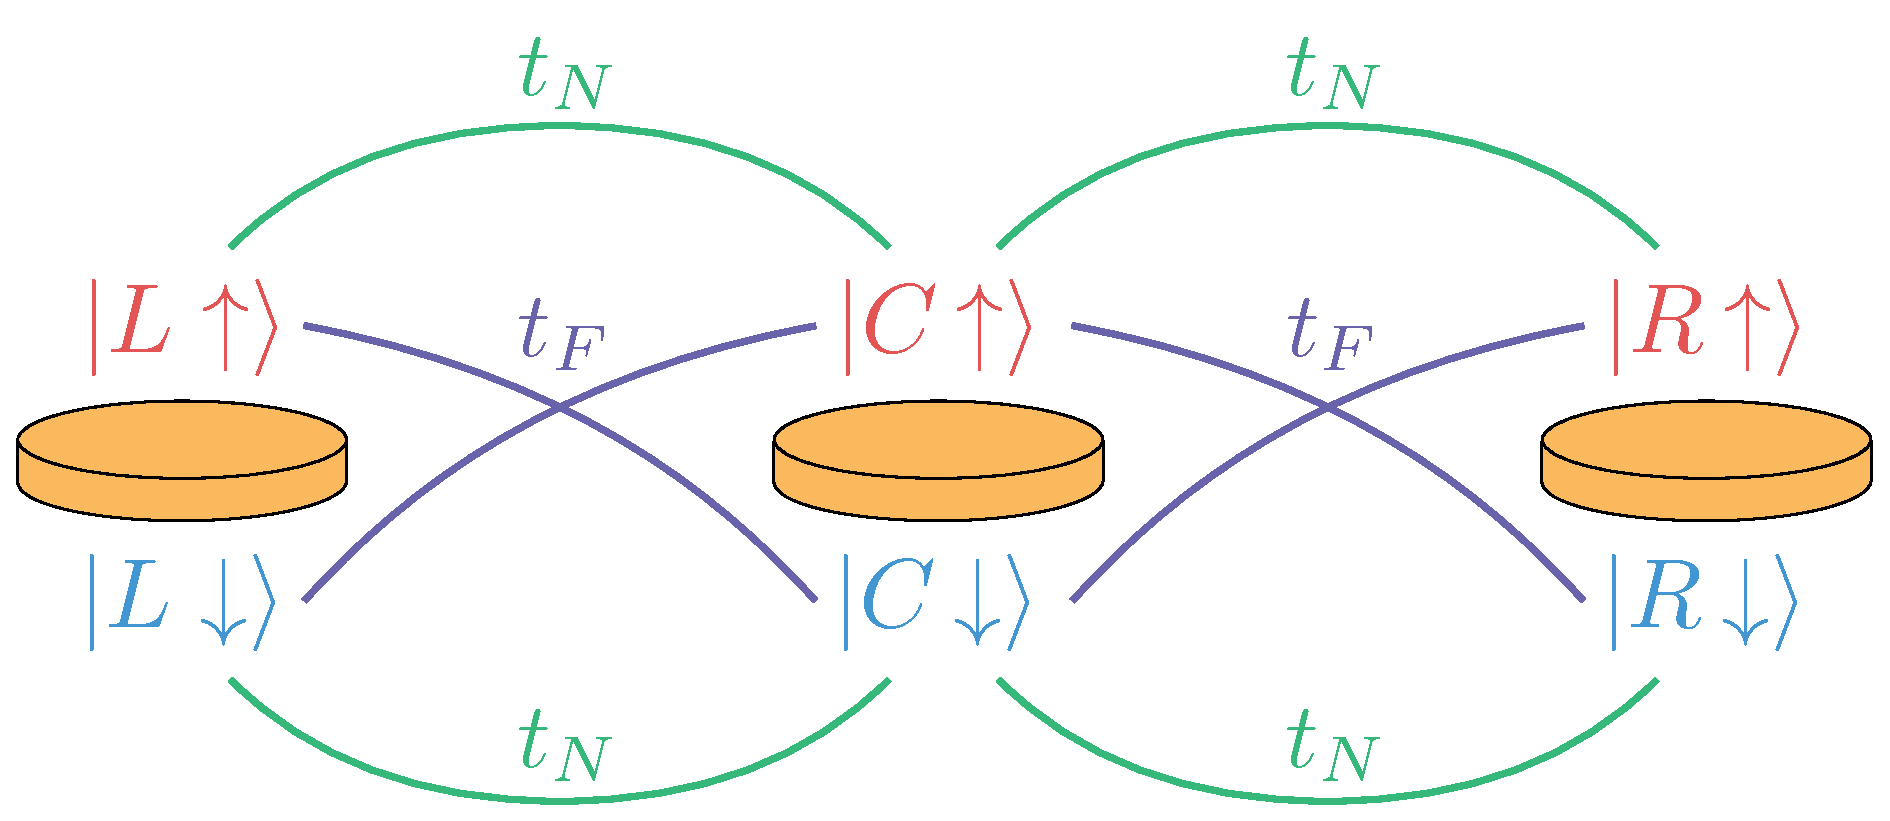
\includegraphics[width=0.5\linewidth]{TQD_Sketch.eps}
	\caption{Pictorial representation for the possible tunneling that a HH can experiment in a linear triple quantum dot array. The spin-conserving and spin-flip tunneling rates are denoted with $t_N$ and $t_F$ respectively. In principle the rates for each dot can be tuned independently.}
	\label{fig:TQD_Sketch}
\end{figure}

Due to the typical energies and times for holes in quantum dots, the units that we will use during this work are $\mu$eV for energy and ns for time. In this units the reduced Plank constant has a value of $\hbar=0.6582 \; \mu$eV$\cdot$ns.


 
% Chapter Template

\chapter{Double Quantum Dot} % Main chapter title

\label{sec:DQD} % Change X to a consecutive number; for referencing this chapter elsewhere, use \ref{ChapterX}

%----------------------------------------------------------------------------------------
%	SECTION 1
%----------------------------------------------------------------------------------------

In this chapter we will focus on the study of a GaAs linear double quantum dot (DQD) array populated with two heavy holes (HH). 

\section{Hamiltonian and eigenstates}
The Hamiltonian of our model is described by Eq.~(\ref{eq:total_Hamiltonian}) which, by explicitly writing down all the terms, corresponds to
\begin{equation}
	\begin{split}
	\hat{\mathcal{H}}_{\text{DQD}}=&\sum_{i}\varepsilon_i\hat{n}_i+\sum_{i}U_i\hat{n}_{i\uparrow}\hat{n}_{i\downarrow}+\frac{1}{2}E_Z\sum_i(\hat{n}_{i\uparrow}-\hat{n}_{i\downarrow})\\
	&-t_N\sum_{\sigma}\left(\hat{c}_{1\sigma}^\dagger c_{2\sigma}+\text{H.c.}\right)-t_F\sum_{\sigma\neq \sigma'}\left(e^{i\theta_{12}}\hat{c}_{1\sigma}^\dagger\hat{c}_{2\sigma'}+\text{H.c.}\right)\; ,
	\end{split}
\end{equation}
where the indices $i=1,2$ denote the left and right dot respectively. We have defined the Zeeman splitting energy as $E_Z\equiv g^*\mu_B B$ with $g^*=1.45$ for holes in GaAs under a perpendicular magnetic field \cite{Bogan2017}. Like electrons, holes statistic is also given by the Fermi-Dirac distribution function, so if we want to obtain a matrix representation of the Hamiltonian we must use the fermionic anti-commutation property
\begin{equation}
\left\{\hat{c}_{i\sigma},\hat{c}_{j\sigma'}\right\}=\delta_{ij}\delta_{\sigma\sigma'}\; .
\end{equation}
With this property we can compute the matrix elements as
\begin{equation}
	\begin{split}
	\bra{\uparrow,\uparrow}\hat{\mathcal{H}}_{\text{DQD}}\ket{\uparrow,\uparrow}=\varepsilon_L+\varepsilon_R+E_Z\; ,
	\end{split}
\end{equation}
and for an off-diagonal element
\begin{equation}
	\begin{split}
	\bra{\uparrow,\uparrow}\hat{\mathcal{H}}_{\text{DQD}}\ket{0,\uparrow\downarrow}&=-t_Fe^{i\theta_{12}}\bra{\uparrow,\uparrow}\hat{c}_{L\uparrow}^\dagger\hat{c}_{R\downarrow}\ket{0,\uparrow\downarrow}\\
	&=-t_Fe^{i\theta_{12}}\bra{0,0}\hat{c}_{R\uparrow}\hat{c}_{L\uparrow}\hat{c}_{L\uparrow}^\dagger \hat{c}_{R\downarrow}\hat{c}_{R\uparrow}^\dagger\hat{c}_{R\downarrow}^\dagger\ket{0,0}\\
	&=-t_Fe^{i\theta_{12}}\bra{0,0}\hat{c}_{R\uparrow}\hat{c}_{R\downarrow}\hat{c}_{R\uparrow}^\dagger \hat{c}_{R\downarrow}^\dagger\ket{0,0}\\
	&=t_Fe^{i\theta_{12}}\bra{0,0}\hat{c}_{R\downarrow} \hat{c}_{R\downarrow}^\dagger\ket{0,0}\\
	&=t_Fe^{i\theta_{12}} \; .
	\end{split}
\end{equation}
With this we can write the Hamiltonian in the atomic basis as
\begin{equation}
	\hat{\mathcal{H}}_{\text{DQD}}=\bordermatrix{~ & \ket{\uparrow,\uparrow} & \ket{\uparrow,\downarrow} & \ket{\downarrow,\uparrow} & \ket{\downarrow,\downarrow} & \ket{\uparrow\downarrow,0} & \ket{0,\uparrow\downarrow}\cr
		~ & \varepsilon_L+\varepsilon_R+E_Z & 0 & 0 & 0 & -t_Fe^{i\theta_{12}} & t_Fe^{i\theta_{12}} \cr
		~ & 0 & \varepsilon_L+\varepsilon_R & 0 & 0 & -t_N & -t_N\cr
		~ & 0 & 0 & \varepsilon_L+\varepsilon_R & 0 & t_N & t_N\cr
		~ & 0 & 0 & 0 & \varepsilon_L+\varepsilon_R -E_Z & t_Fe^{i\theta_{12}} & -t_Fe^{i\theta_{12}}\cr
		~ & -t_Fe^{-i\theta_{12}} & -t_N & t_N & t_Fe^{-i\theta_{12}} &  2\varepsilon_L+U_L & 0 \cr
		~ & t_Fe^{-i\theta_{12}} & -t_N & t_N & -t_Fe^{-i\theta_{12}} &  0 & 2\varepsilon_R+U_R \cr}\; .
\end{equation}
In the experimental devices is typical to tune the intradot Coulomb interaction to be much greater in one dot than in the other one $U_L\gg U_R=U$ so we will work with the Hilbert subspace in which $\ket{\uparrow\downarrow,0}$ is not included. In this kind of systems the atomic basis in not the typical choice, so we change to the molecular basis Eq.~(\ref{eq:molecular_basis}) and the Hamiltonian reads as
\begin{equation}
\hat{\mathcal{H}}_{\text{DQD}}=\bordermatrix{~ & \ket{T_+(1,1)} & \ket{T_0(1,1)} & \ket{T_-(1,1)} & \ket{S(0,2)} & \ket{S(1,1)}\cr
	~ & E_Z & 0 & 0 & t_Fe^{i\theta_{12}} & 0 \cr
	~ & 0 & 0 & 0 & 0 & 0\cr
	~ & 0 & 0 & -E_Z & -t_Fe^{i\theta_{12}} & 0 \cr
	~ & t_Fe^{-i\theta_{12}} & 0 & -t_Fe^{-i\theta_{12}} & 2\varepsilon_R+U & -\sqrt{2}t_N \cr
	~ & 0 & 0 & 0 & -\sqrt{2}t_N &  \varepsilon_L+\varepsilon_R  \cr}\; .
\label{eq:Hamiltonain_DQD_2HH_Full}
\end{equation}
Here we can see that the triplet state $\ket{T_0(1,1)}$ is not coupled to any other state, so it will not be considered for the rest of the chapter. Furthermore, if the magnetic field is high enough we can also neglect $\ket{T_+(1,1)}$. The detuning between dots is defined as $\varepsilon\equiv \varepsilon_R-\varepsilon_L$, in order to decrease the number of free parameters we fix $\varepsilon_L=-\varepsilon_R$, so the final effective Hamiltonian is
\begin{equation}
\hat{\mathcal{H}}_{\text{DQD}}^{\text{eff.}}=\bordermatrix{~ & \ket{T_-(1,1)} & \ket{S(0,2)} & \ket{S(1,1)}\cr
	~ & -E_Z & -t_Fe^{-i\theta_{12}} & 0 \cr
	~ & -t_Fe^{-i\theta_{12}} & \varepsilon +U & -\sqrt{2}t_N \cr
	~ & 0 & -\sqrt{2}t_N &  0  \cr}\; .
\label{eq:effective_Hamiltonian_DQD}
\end{equation}
The characteristic polynomial of this matrix corresponds to
\begin{equation}
	\abs{\hat{\mathcal{H}}_{\text{DQD}}^{\text{eff.}}-\lambda\mathds{1}}=(\varepsilon+U-\lambda)\lambda^2+\lambda\left[(\varepsilon+U-\lambda)E_Z+t_F^2\right]+2(\lambda+E_Z)t_N^2=0\; ,
\end{equation}
which has no dependence on the complex phase se we set $\theta_{12}=0$ for the rest of the work. Let us denote with $\ket{\phi_i}$ the instant eigenstates and $E_i$ the energies of the system whose spectrum can be found in Fig.~\ref{fig:eigenenergies_DQD_2HH}. This energy spectrum corresponds to the Hamiltonian given in Eq.~(\ref{eq:Hamiltonain_DQD_2HH_Full}), before neglecting the two triplet states commented above. In order to fix a notation we will denote with $\ket{\phi_0}$ the lowest energy state (blue), $\ket{\phi_1}$ the first excited state (red) and so on up to $\ket{\phi_4}$ (purple) for the most energetic instant state. The results coincide with those obtained by other experimental groups \cite{SachrajdaUnpublished}.
\begin{figure}[!htbp]
	\centering
	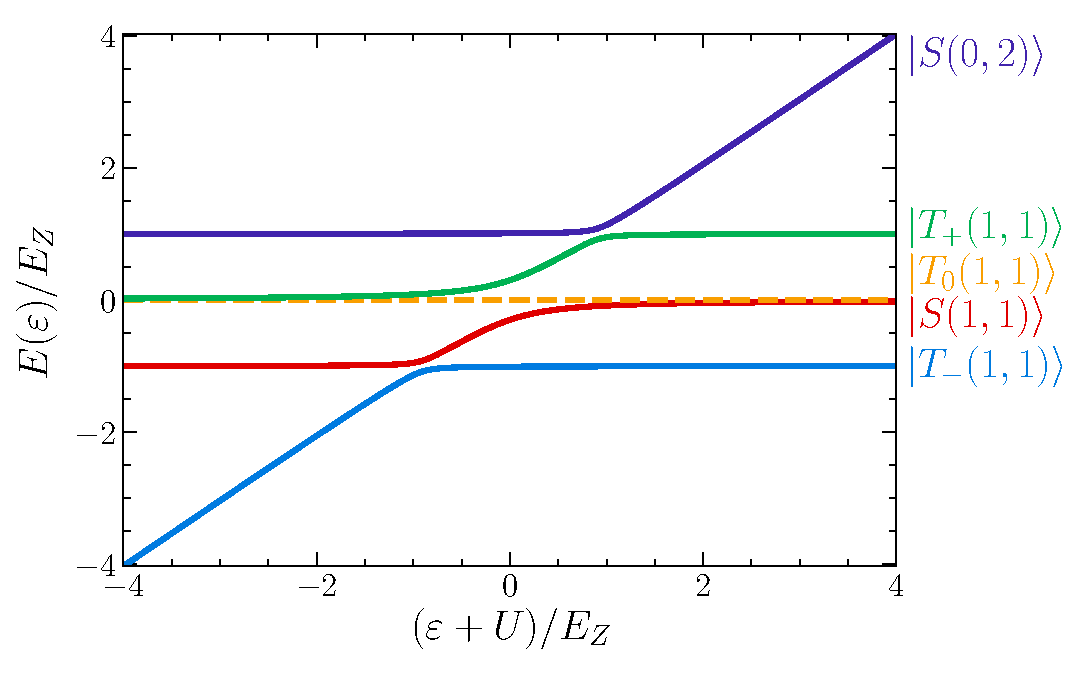
\includegraphics[width=0.8\linewidth]{eigenenergies_DQD_2HH.eps}
	\caption{Energy spectrum for a GaAs DQD populated with two HH. The parameters used are $E_Z=1.17\; \mu$eV, $U=2$ meV, $t_N=0.25\; \mu$eV and $t_F=0.1\; \mu$eV. At the right of each instant state we have specified the corresponding element in the molecular basis in the high detuning limit.}
	\label{fig:eigenenergies_DQD_2HH}
\end{figure}

Our aim in this chapter is to find a protocol with which the system can be transferred from the triplet state $\ket{T_-(1,1)}$ to the single occupation singlet state $\ket{S(1,1)}$. This transition can be obtained  throughout the adiabatic state $\ket{\phi_1}$ by varying the detuning of the QD's from $(\varepsilon+U)\ll-E_Z$ to $(\varepsilon+U)\gg E_Z$ as can be seen in the energy spectrum. In our model we have not included any term that allows the spin flip of a particle without tunneling to the other dot, so the only possible path is
\begin{equation}
	\ket{\downarrow,\downarrow}\rightarrow\ket{0,\uparrow\downarrow}\rightarrow\frac{1}{\sqrt{2}}(\ket{\uparrow,\downarrow}-\ket{\downarrow,\uparrow})\; .
\end{equation}
But this transitions has the inconvenience that the charge changes its location, producing the undesired charge noise. We could mitigate this effect if we could find an instant eigenstate which has no weight if the double occupation state, also known as dark state. The adiabatic state can be written generically as
\begin{equation}
	\ket{\phi_1}=a_1\ket{S(1,1)}+a_2\ket{S(0,2)}+a_3\ket{T_-(1,1)}\; .
	\label{eq:adiabatic_state}
\end{equation}
The eigenstates have not a simple analytical solution, so we have opted to find the dark state by solving numerically the instant eigenstates of the system. There are many different variables in the system so we fix the Coulomb interaction $U$ and the Zeeman splitting $E_Z$, and change the detuning $\varepsilon$ and the spin-conserving tunneling rate $t_N$. The spin-flip tunneling rate can be experimentally tune independently of $t_N$, in this chapter we will restrict ourselves to a constant value of $t_F=0.1\; \mu$eV, what is in line with some experimental data \cite{Bogan2018}. The numerical results for the the population of the double occupation singlet state ($\abs{a_2}^2$ in Eq.~(\ref{eq:adiabatic_state})) in terms of the detuning and the tunneling rate are shown in Fig.~\ref{fig:occupation_middle_state}. As we have said before, the desired transference is only achievable if the detuning goes from $(\varepsilon+U)\ll -E_Z$ to $(\varepsilon+U)\gg 0$. This means that if we want to suppress the population of the double occupation singlet state during the transference we must set a high spin-conserving tunneling rate $t_N\sim 5\mu$eV.
\begin{figure}[!htb]
	\centering
	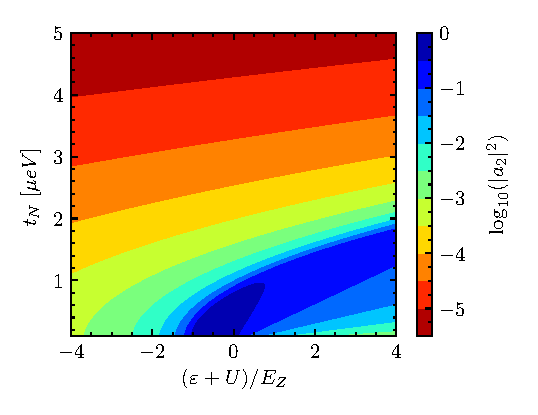
\includegraphics[width=0.6\linewidth]{occupation_middle_state.eps}
	\caption{Population of the double occupied singlet state $\ket{S(0,2)}$ in the first excited instant state $\ket{\phi_1}$, where we have defined $\abs{a_2}^2\equiv \abs{\braket{S(0,2)}{\phi_2}}^2$. All the other parameters are the same than in Fig.~\ref{fig:eigenenergies_DQD_2HH}.}
	\label{fig:occupation_middle_state}
\end{figure}

Other aspect that is worth to discuss is the initial and final values for the detuning. The ideal scenario would be that the adiabatic state corresponds to the target states at the beginning and the end of the protocol, i.e. $\ket{\phi_1(t=0)}=\ket{T_-(1,1)}$ and $\ket{\phi_1(t=t_f)}=\ket{S(1,1)}$, but this is only possible in the asymptotic limit $\varepsilon:[-\infty,+\infty]$, what is impossible to achieve experimentally. The values for $\abs{a_1}^2$ and $\abs{a_3}^2$ in terms of the detuning and the tunneling $t_N$ are shown in Fig.~\ref{fig:limits_FAQUAD}. Note that what is represented is the not exactly the population but how close its to the unity in logarithmic scale. Here we can see that when we increase the value for the tunneling rate in order not to populate the double occupied singlet state, and fixed the values $\abs{a_3(t=0)}^2$ and $\abs{a_1(t=t_f)}^2$, the total range for the detuning becomes wider which results in a higher energy expenditure. We must find a equilibrium between high fidelities and a reasonable limits for the detuning, this is why for the rest fo the chapter set the initial and final detuning values such that $\abs{a_3(t=0)}^2=0.9999$ and $\abs{a_1(t=t_f)}^2=0.9999$. If better fidelity is needed we can always  increase the range used for detuning.\\
\begin{figure}[!htb]
	\centering
	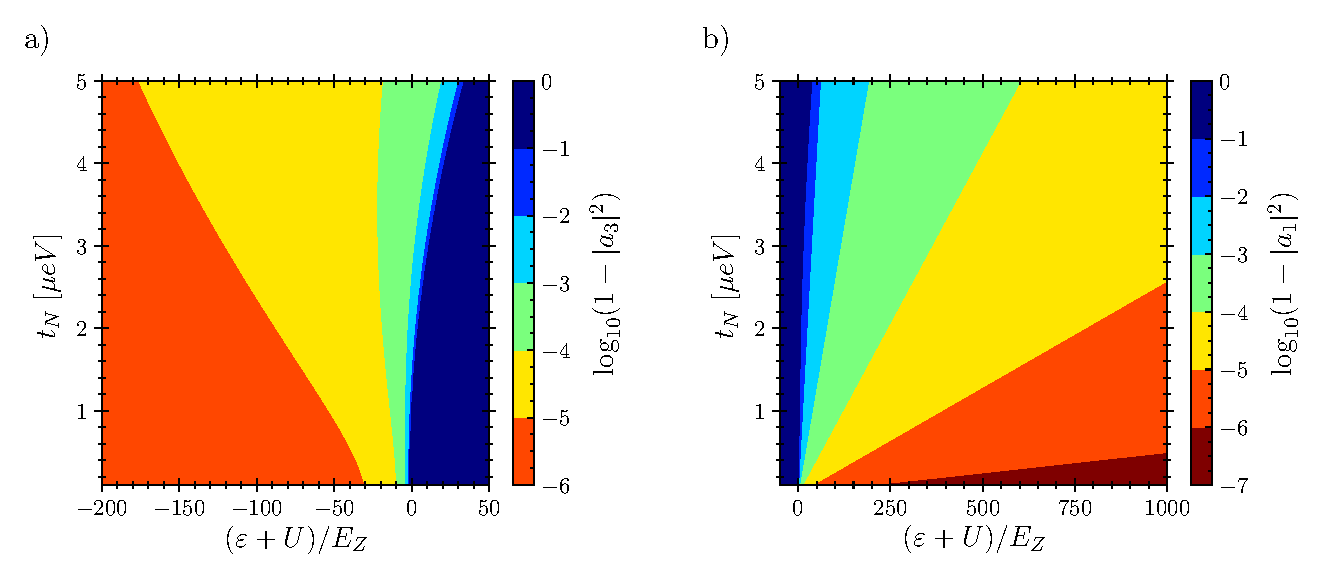
\includegraphics[width=0.93\linewidth]{limits_FAQUAD.eps}
	\caption{Population of a) the triplet state and b) the single occupied singlet state in terms of the detuning and the spin-conserving tunneling rate. All the other parameters are the same than in Fig.~\ref{fig:eigenenergies_DQD_2HH}.}
	\label{fig:limits_FAQUAD}
\end{figure}

Now we must choose what STA scheme we will use in the system. As we have mentioned before it is not easy to obtain an analytical expression for the three instant eigenvectors so we rule out the use of CD. We are dealing with a three level system what means that the eigenstates can be conveniently obtained numerically and considering that with these we obtain all the information in the system we decided to go for the use of FAQUAD.

\section{FAQUAD Results}
The parameters that we will use are a Zeeman splitting of $E_Z=1.17\: \mu$eV, which corresponds to a magnetic field $B\sim 15$ mT, an intradot Coulomb interaction of $U= 2$ meV, and a spin-flip tunnelling rate of $t_F=0.1\; \mu$eV. Let's start choosing a moderate value for the spin-conserving tunnelling rate of $t_N=0.25\; \mu$eV with which the double occupied singlet will be occupied. This will serve us as a first test to verify that FAQUAD protocol achieves the target state with fidelities close to the unit. In the following we will use the definition for the adimensional detuning $\tilde{\varepsilon}\equiv (\varepsilon+U)/E_Z$ to shorten the notation in the text, although the original notation will be retained in the figures for clarity. With the above values for the parameters of the system we can compute numerically the initial and final detuning to obtain $\abs{a_1(t=0)}^2=\abs{a_3(t=t_f)}^2=0.9999$ obtaining $\tilde{\varepsilon}(t=0)=-10.08$ and $\tilde{\varepsilon}(t=t_f)=30.15$. Together with the eigenstates and eigenenergies that we can obtain numerically we can introduce them in Eq.~(\ref{eq:c_tilde_deff}) identifying $\lambda(t)=\varepsilon(t)$ and the initial state as $\ket{\phi_1}$, by which we want to perform the adiabatic transfer. With this we obtain a value for the rescaled adiabatic parameter $\tilde{c}=4.34$ ns, so if we want an adiabatic passage $c=\tilde{c}/t_f\ll 1$ we need times $t_f\sim 100$ ns. Now introducing this factor in Eq.~(\ref{eq:parameter_ODE_2}) we can solve by numerical integration the dependence of the detuning with the rescaled time $s\equiv t/t_f$, what is shown in Fig.~\ref{fig:FAQUAD_detuning_2QD_2HH} a). What is more interesting is how the rate of change, i.e the speed, of the detuning varies as we approach or move away from the avoided crossings. In Fig.~\ref{fig:FAQUAD_detuning_2QD_2HH} b) we can see that near $\tilde{\varepsilon}=-1$ and $\tilde{\varepsilon}=0$, where avoided crossings are located, the detuning slows down to ensure an adiabatic passage. Nevertheless, as the energies are away from each other the detuning speeds up to get the shortest possible final times. The obtained shape is smooth so the detuning implementation in a real life experiment is feasible.
\begin{figure}[!htbp]
	\centering
	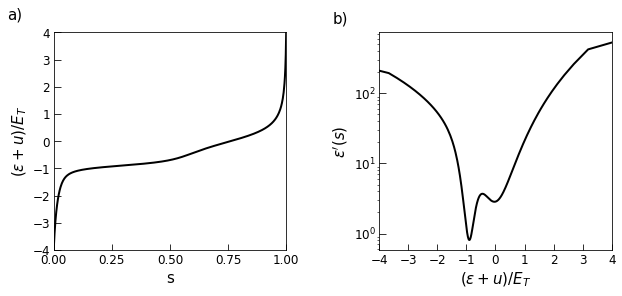
\includegraphics[width=0.9\linewidth]{FAQUAD_detuning_2QD_2HH.pdf}
	\caption{a) Dependence of the detuning in terms of the rescaled time $s=t/t_f$ obtained by solving numerically the FAQUAD protocol. b) Derivative of the detuning in terms of the detuning itself. The spin-conserving tunnelling used is $t_N=0.25\; \mu$eV, all the other parameters are the same than in Fig.~\ref{fig:eigenenergies_DQD_2HH}.}
	\label{fig:FAQUAD_detuning_2QD_2HH}
\end{figure}

Let's define the fidelity of the protocol as
\begin{equation}
	\mathcal{F}(t_f)\equiv \abs{\braket{\phi_1(t_f)}{\Psi(t_f)}}^2\; ,
\end{equation}
where $\ket{\Psi(t)}$ represent the solution of the time dependent Schrödinger equation. We solve the density matrix dynamics equation for several final times, what is shown in Fig.~\ref{fig:FAQUAD_2QD_Results}, the dashed red line represents the lower bound for the fidelity given by Eq.~(\ref{eq:lower_bound_fidelity}). As we have predicted by adiabatic perturbation theory Eq.~(\ref{eq:FAQUAD_fidelity}), the fidelity has a wavy behaviour governed by two frequencies. As the final time grows the fidelity is stabilized at a value close to unity. Using Eq.~(\ref{eq:FAQUAD_frecuencies}) we predict two periods of $T_1=10.45$ ns and $T_2=3.66$ ns. Both oscillations can be seen in the fidelity, but in order to obtain a more precise value for the periods of each oscillation we can numerically compute the Fourier transform for the fidelity Fig.~\ref{fig:frecuency_spectrum}. We can observe that the predicted values for the frequency are close to the real ones, but we obtain more than two peaks in the frequency spectrum. These new oscillations can be analytically computed used higher orders in adiabatic perturbation theory.
\begin{figure}[!htb]
	\centering
	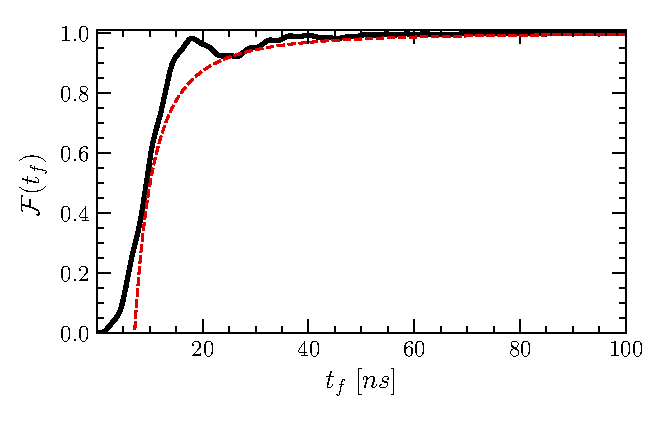
\includegraphics[width=0.7\linewidth]{FAQUAD_2QD_Results.eps}
	\caption{Fidelity in term of the final time. The spin-conserving tunnelling used is $t_N=0.25\; \mu$eV, all the other parameters are the same than in Fig.~\ref{fig:eigenenergies_DQD_2HH}. The red dashed line represent the lower bound for the fidelity predicted adiabatic perturbation theory at first order.}
	\label{fig:FAQUAD_2QD_Results}
\end{figure}
\begin{figure}[!htb]
	\centering
	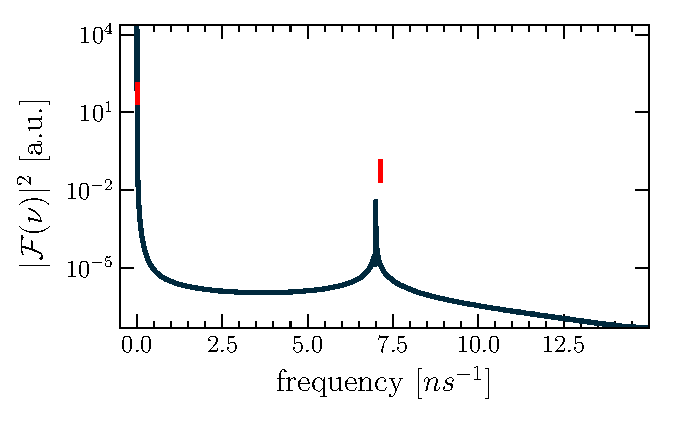
\includegraphics[width=0.7\linewidth]{frecuency_spectrum.eps}
	\caption{Fourier transform in arbitrary units for the fidelity shown in Fig.~\ref{fig:FAQUAD_2QD_Results}. The two red lines corresponds to the frequencies predicted at first order in adiabatic perturbation theory.}
	\label{fig:frecuency_spectrum}
\end{figure}

The first peak of the fidelity is reached at $t_f=18.03$ ns, obtaining a value of $\mathcal{F}=0.98$. The evolution of the states at this final time can be seen in Fig.~\ref{fig:states_evolution_1}. The target state $\ket{S(1,1)}$ is reached at the end of the passage, but in the meantime the double occupation singlet state has a population considerably high. The maximum population of this state for the other peaks in the fidelity are no lower, reaching values of $\abs{\braket{S(0,2)}{\Psi(t_f)}}^2\sim 0.8$.
\begin{figure}[!htb]
	\centering
	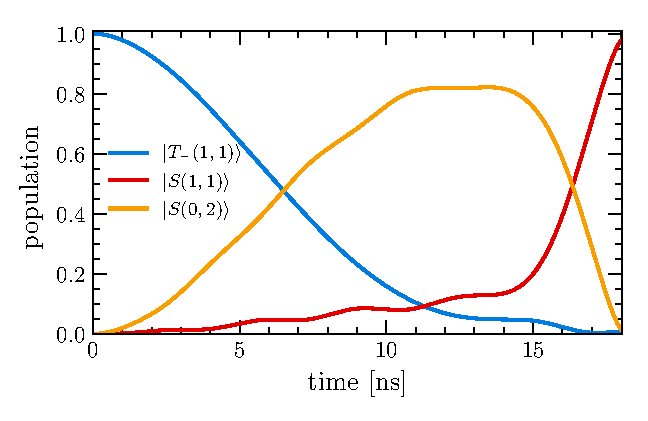
\includegraphics[width=0.7\linewidth]{states_evolution_1.eps}
	\caption{Population for the different states during the protocol with a final time of $t_f=18.03$ ns. The fidelity at this time is $\mathcal{F}=0.98$. The spin-conserving tunnelling used is $t_N=0.25\; \mu$eV, all the other parameters are the same than in Fig.~\ref{fig:eigenenergies_DQD_2HH}.}
	\label{fig:states_evolution_1}
\end{figure}



In order to decrease the population of $\ket{S(0,2)}$ we must use higher values for the spin-conserving tunneling rates as we have seen in Fig.~\ref{fig:occupation_middle_state}, let's use for instance $t_N=5\; \mu$eV. In order to keep the initial and final populations in the adiabatic state of $\abs{a_1(t=0)}^2=0.9999$ and $\abs{a_3(t=t_f)}^2=0.9999$ we must increase the range for the detuning. With the new tunneling rates we obtain that $\tilde{\varepsilon}(0)=-18.18$ and $\tilde{\varepsilon}(t_f)=619.21$ for the initial and final time respectively. With this parameters we obtain $\tilde{c}=21.42$ ns, so the final times must be greater than those previously used with a smaller tunneling rate. In Fig.~\ref{fig:FAQUAD_detuning_2QD_2HH_2} we have shown the detuning and its derivative. The qualitative behaviour is very similar to that obtained previously in Fig.~\ref{fig:FAQUAD_detuning_2QD_2HH}, with the difference that now the two avoided crossings are so close to each other that we only appreciate one minimum in the derivative.
\begin{figure}[!htb]
	\centering
	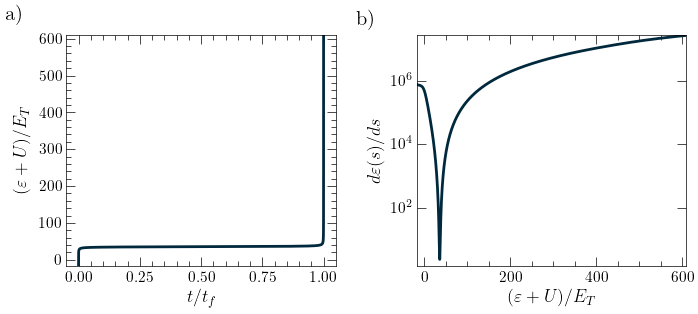
\includegraphics[width=0.92\linewidth]{FAQUAD_detuning_2QD_2HH_2.pdf}
	\caption{a) Dependence of the detuning in terms of the rescaled time $s=t/t_f$ obtained by solving numerically the FAQUAD protocol. b) Derivative of the detuning in terms of the detuning itself. The spin-conserving tunnelling used is $t_N=5\; \mu$eV, all the other parameters are the same than in Fig.~\ref{fig:eigenenergies_DQD_2HH}.}
	\label{fig:FAQUAD_detuning_2QD_2HH_2}
\end{figure}

The fidelity for $t_N=5 \; \mu$eV is shown in Fig.~\ref{fig:FAQUAD_2QD_Results_2}. Here the amplitudes of the high frequency oscillations are smaller than the width of the line, so can not be seen. However, computing again the Fourier transformation (not shown here) reveals that the values obtained are in line with what we get using Eq.~(\ref{eq:FAQUAD_frecuencies}). As we have predicted the total time needed for reaching the first peak, $t_f=74.11$ ns, is much larger than before. However, the fidelity has improved reaching a value of $\mathcal{F}=0.99998$ at the first peak.

\begin{figure}[!htb]
	\centering
	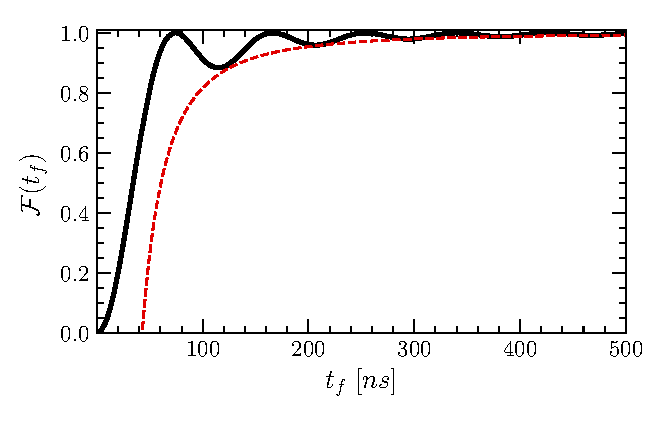
\includegraphics[width=0.7\linewidth]{FAQUAD_2QD_Results_2.eps}
	\caption{Fidelity in term of the final time. The spin-conserving tunnelling used is $t_N=5\; \mu$eV, all the other parameters are the same than in Fig.~\ref{fig:eigenenergies_DQD_2HH}. The red dashed line represent the lower bound limit for the fidelity predicted adiabatic perturbation theory at first order.}
	\label{fig:FAQUAD_2QD_Results_2}
\end{figure}

The purpose of increasing the spin-conserving tunneling rate was to mitigate the charge noise by decreasing the total population of the double occupation singlet state $\ket{S(0,2)}$. In Fig.~\ref{fig:states_evolution_2} we have plotted the evolution for the different states of the system for a total time corresponding to the first peak in the fidelity. We can see that the population of $\ket{S(0,2)}$ has decreased with respect to a lower tunneling rate, obtaining a maximum value of $2.5\%$ during the transference. This value remains constant for all other peaks in fidelity.
\begin{figure}[!htb]
	\centering
	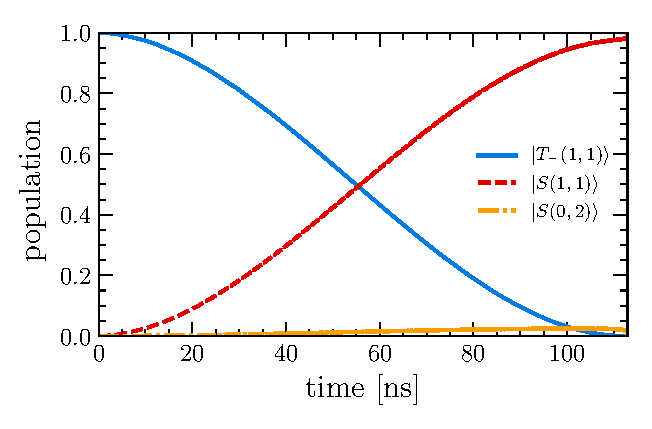
\includegraphics[width=0.7\linewidth]{states_evolution_2.eps}
	\caption{Population for the different states during the protocol with a final time of $t_f=74.11$ ns. The fidelity at this time is $\mathcal{F}=0.99998$. The spin-conserving tunnelling used is $t_N=5\; \mu$eV, all the other parameters are the same than in Fig.~\ref{fig:eigenenergies_DQD_2HH}.}
	\label{fig:states_evolution_2}
\end{figure}

All the results that we have given so far was obtained by using the effective Hamiltonian shown in Eq.~(\ref{eq:effective_Hamiltonian_DQD}). We can include the triplet state $\ket{T_+(1,1)}$ and repeat the FAQUAD protocol now with three terms in the summatory of Eq.~(\ref{eq:parameter_ODE_2}). Computing the fidelity obtained in terms of the total time we get that the first peak is reached at $t_f=105.6$ ns, a slightly quicker than when working with the effective Hamiltonian. The fidelity in this peak corresponds to $\mathcal{F}=0.99990$, way to close to the previously value. The time evolution of the system (not shown here) is also quite similar to when we only deal with a three level system, so the use of the effective Hamiltonian is justified. In order to save computation time we will stick to this effective model for the rest of the chapter.


\section{One qubit gate}
Now that we have been able to achieve a negligible population in the double occupation singlet state, we are dealing with a two level system, so the map with a qubit is natural. Let's call $\ket{0}\equiv\ket{T_-(1,1)}$ and $\ket{1}\equiv \ket{S(1,1)}$ the computational basis. In order to represent the two degrees of freedom present in a qubit it's usual to work with the Bloch sphere, in which each pole represent a element of the computation basis. The superposition of $\ket{0}$ and $\ket{1}$ is given by the polar angle $0\leq \theta\leq \pi$, and the azimuthal angle $0\leq\phi<2\pi$. A general wave function can be written as
\begin{equation}
	\ket{\psi}=r\cos(\theta/2)\ket{0}+e^{i\phi}\sin(\theta/2)\ket{1}\; ,
\end{equation}
where we have introduced the radius $0<r\leq 1$ to take into account a possible leakage out of the computation basis
\begin{equation}
	r\equiv \abs{\braket{\Psi(t_f)}{T_-(1,1)}}^2+\abs{\braket{\Psi(t_f)}{S(1,1)}}^2\; .
\end{equation}
In Fig.~\ref{fig:Bloch_sphere_combined} a) we have plotted the trajectory in the Bloch sphere followed by the system as the total time for the FAQUAD protocol varies.
\begin{figure}[!htb]
	\centering
	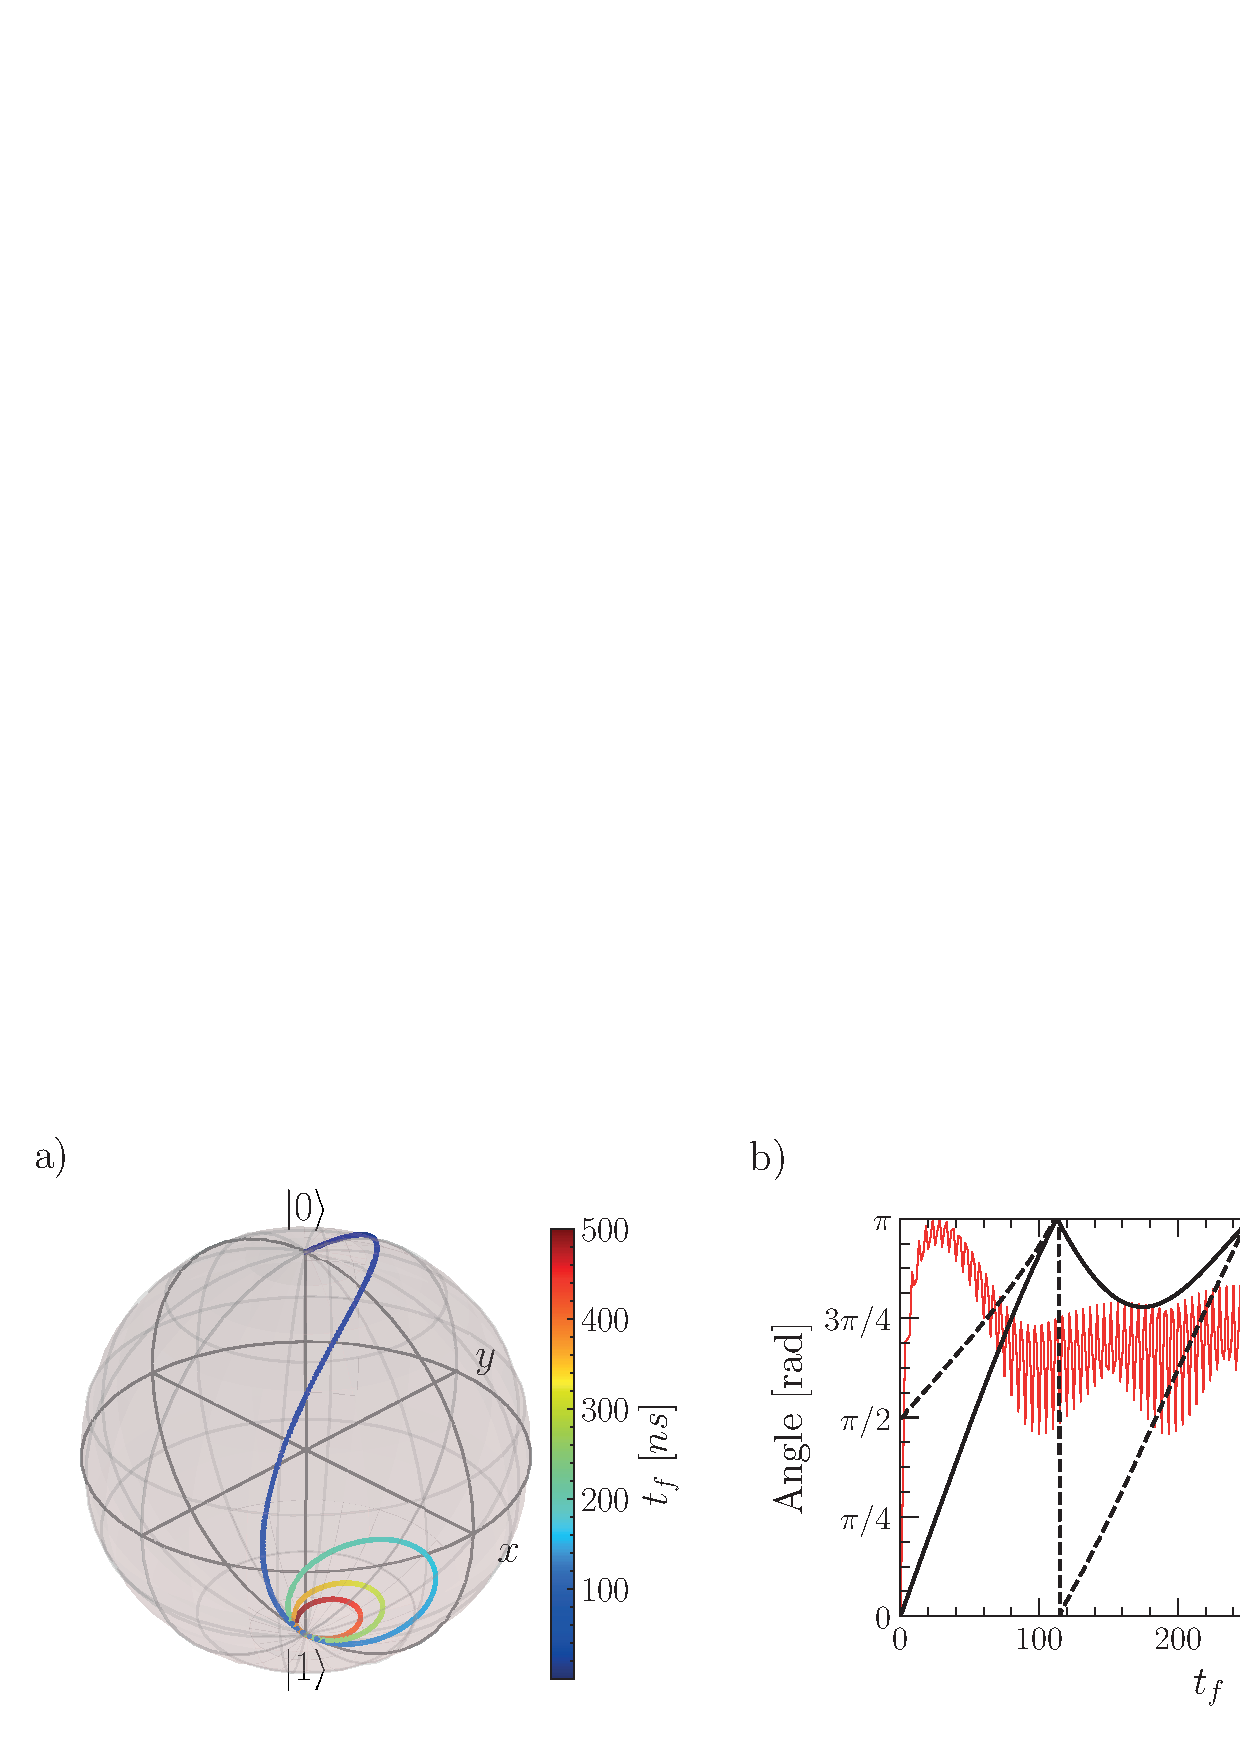
\includegraphics[width=\linewidth]{Bloch_sphere_combined.pdf}
	\caption{a) Trajectory for the system in the Bloch sphere in terms of the final time. We have identified $\ket{0}\equiv\ket{T_-(1,1)}$ and $\ket{1}\equiv \ket{S(1,1)}$. b) Evolution for the polar angle $\theta$ (solid black), the azimuthal angle (dashed black) $\phi$ and the radius (solid red). The spin-conserving tunnelling used is $t_N=5\; \mu$eV, all the other parameters are the same than in Fig.~\ref{fig:eigenenergies_DQD_2HH}.}
	\label{fig:Bloch_sphere_combined}
\end{figure}

We are able to rotate a state from the north pole $\ket{0}$ to the south pole $\ket{1}$ including all intermediate values of the polar angle. This angle can be modified vie the final time $t_f$, Fig.~\ref{fig:Bloch_sphere_combined}, so we have total control over this parameter. To be able to reach any point on the sphere of Bloch we must be able to rotate a state on the z axis, what can be done by letting the system evolve with a time independent Hamiltonian, the acquired phase can be written as
\begin{equation}
	\phi_a(t)=-\frac{1}{\hbar}\int_0^t dt'[E_{S(1,1)}-E_{T_-(1,1)}]=-\frac{E_Z}{\hbar}t\; .
\end{equation}
The maximum acquired phase that we must need is $\phi_a=2\pi$, which can be achieved in a time $t=2\pi\hbar/E_Z$. Using a value of $E_Z=1.17\; \mu$eV this corresponds to a time of $t=3.5$ ns. This rotation can be speed up or slow down by decreasing or increasing the magnetic field respectively. Then we have total control over $\theta$ and $\phi$, so we can prepare our qubit in an arbitrary state in at most $120$ ns. This constitutes an universal one qubit quantum gate. The dependences of $\theta$ and $\phi$ with the total time $t_f$ has a really simple behaviour and can be fitted by a first or second order polynomial function, so it's easy to extract the time needed to achieved a certain value. Possible leaks outside the computation base are limited to $\max[(1-r)^2]=6.4\times10^{-3}\%$ at most, as shown in Fig.~\ref{fig:Bloch_sphere_combined} b) (red).
\section{Systematic and stochastic errors}
 

%----------------------------------------------------------------------------------------
%	THESIS CONTENT - APPENDICES
%----------------------------------------------------------------------------------------

\appendix % Cue to tell LaTeX that the following "chapters" are Appendices

% Include the appendices of the thesis as separate files from the Appendices folder
% Uncomment the lines as you write the Appendices

% Appendix A

\chapter{Density Matrix} % Main appendix title

\label{app:Density_Matrix} % For referencing this appendix elsewhere, use \ref{AppendixA}


% Appendix Template

\chapter{Computational Methods} % Main appendix title

\label{app:Numerical_methods} % Change X to a consecutive letter; for referencing this appendix elsewhere, use \ref{AppendixX}

In this appendix we will show some of the numerical methods used in this work. We also present some fragments of the code written to obtain the results given in Chapters \ref{sec:DQD} and \ref{sec:TQD}. Two different programming languages has been used, on one hand we have used Wolfram Mathematica 12.0 for the analytical computations like the obtention of the eigenvectors of a given Hamiltonian. This is necessary for finding the dark state shown in Chapter \ref{sec:TQD} and the obtention of the counteradiabatic driving Hamiltonian. Lastly this software was used to solve the system of ODE's. All the code is written with build-in functions, so the syntax is extremely simpler and is not worth to show here some examples.

On the other hand, we have used Python 3.7 for the rest of the calculations, here is where the core of this work is located. All the code written tries to be the more general as possible, so we can reuse it on future works. In Chapter \ref{sec:DQD} we have used the FAQUAD protocol, for which we need to solve Eq.~(\ref{eq:c_tilde_deff}). The function to compute $\tilde{c}$ needs as input and array with the equally spaced values of the parameter $\lambda$, the eigenstates and eigenenergies and the index index for the initial adiabatic state. We can also specify the value for the reduced Plank constant $\hbar$ and a matrix denoting the derivative $\partial_\lambda \hat{\mathcal{H}}/\partial\lambda$. When computing the numerical derivative the precision is low if the step is not small enough. This is why we perform a filter for the final result mitigating this problem.
\begin{mintedbox}{python}
import numpy as np
from scipy.integrate import romb
from scipy.constants import h, e
from scipy.signal import medfilt
	
hbar_muev_ns = ((h / e) / (2 * np.pi)) * 10 ** 6 * 10 ** 9
	
def compute_adiabatic_parameter(x_vec, states, energies, initial_state, hbar=hbar_muev_ns, partial_Hamiltonian=None):
	"""
	Compute the factors need for the FAQUAD and the value of tilde{c}.
	:param x_vec: (numpy.array) Vectors with the values of the parameters we are interested to change with a total of N values
	:param states: (numpy.matrix) Matrix with the D instant eigenstates of the system. The dimension is [N x D x D]
	:param energies: (numpy.matrix) Matrix with the D instant eigenenergies of the system. The dimension is [N x D]
	:param initial_state: (int) Index for the initial state in which we begin the protocol
	:param hbar: (float) Value for hbar
		:param partial_Hamiltonian: (numpy.matrix) Matrix with the derivative of the Hamiltonian
	:return: (list) List with the factors computed and the value of c_tilde.
	"""
	n, dim = np.shape(energies)

	if partial_Hamiltonian is None:
		method_1 = True
	else:
	method_1 = False
	
	if method_1:
		derivatives = np.zeros([n, dim, dim], dtype=complex)
		for i in range(0, dim): 
			for j in range(0, dim):
				derivatives[:, j, i] = np.gradient(states[:, j, i], x_vec)
	
	counter = 0
	factors = np.zeros([n, dim - 1])
	for i in range(0, dim):
		if i != initial_state:
			if method_1:
				factors[:, counter] = np.abs(np.sum(np.conjugate(states[:, :, initial_state]) * derivatives[:, :, i], axis=1) / (energies[:, initial_state] - energies[:, i]))
			else:
				for k in range(0, n):
					factors[k, counter] = np.abs(np.matmul(np.matmul(
					np.conjugate(states[k, :, i]), partial_Hamiltonian[k, :, :]), states[k, :, initial_state]) / (energies[k, i] - energies[k, initial_state]) ** 2)
			counter += 1
	
	if method_1:
		for i in range(0, dim - 1):
			factors[:, i] = medfilt(factors[:, i], 5)
	
	
	c_tilde = hbar * np.sum(romb(factors, dx=np.abs(x_vec[0] - x_vec[1]), axis=0))
	
	return factors, c_tilde
\end{mintedbox}

One we have the value for $\tilde{c}$ we must numerically solve the ODE that give us the time dependence of the parameter $\lambda(t)$, Eq.~(\ref{eq:parameter_ODE_2}), Here we can reuse some factors obtained by the previous function. Here there can occur that due to numerical errors in the differential equation solver the boundary condition is not satisfied $\tilde{\lambda}(s=1)=\lambda(t=t_f)$, so we allow that the final value for the parameter is reached at $s\sim 1$. After that we force the correct boundary condition by interpolating the function.
\begin{mintedbox}{python}
from scipy.interpolate import interp1d
from scipy.integrate import odeint
	
def compute_parameters_interpolation(x_vec, factors, c_tilde, nt=None, hbar=hbar_muev_ns):
	"""
	Function to solve the ODE which gives the result for the parameters in terms of the adimensional variable s=[0,1] for the FAQUAD protocol
	:param x_vec: (numpy.array) Vector with the values of the independent variable
	:param factors: (numpy.matrix) Matrix with the factors of the FAQUAD protocol
	:param c_tilde: (float) Value for the rescaled adiabatic parameter
	:param nt: Number of steps for the time variable
	:param hbar: Value for h bar
	:return: Vector of times and the parameter
	"""
	sig = np.sign(x_vec[1] - x_vec[0])

	if nt is None:
		nt = len(x_vec)

	def factor_interpolation(x):
		return interp1d(x_vec, 1 / np.sum(factors, axis=1), kind='quadratic', fill_value="extrapolate")(x)

	def model(y, _):
		return sig * c_tilde / hbar * factor_interpolation(y)

	s_max = 1
	s = np.linspace(0, s_max, nt, endpoint=True)

	counter = 0
	reached = False
	while not reached:
		x_sol = odeint(model, x_vec[0], s)[:, 0]
		counter += 1
		if np.any(sig * x_sol > sig * x_vec[-1]):
			index_max = np.where(sig * x_sol > sig * x_vec[-1])[0][0]
			reached = True
		else:
			s *= 1.1

		if counter > 20:
			print('The limit value has not been reached.')
			return ()

	s = np.linspace(0, 1, index_max + 1)
	x_sol = x_sol[:index_max + 1]
	x_sol = interp1d(s, xsol)

	return s, x_sol
\end{mintedbox}

Other relevant value for the FAQUAD scheme is the frequency of oscillation for the fidelity, Eq.~(\ref{eq:FAQUAD_frecuencies}). Here we have to identify which is the time dependent parameter, compute the eigenenergies and obtain the integral for each frequency.
\begin{mintedbox}{python}
def compute_periods(x_sol, hamiltonian, parameters, hbar, index, state):
	"""
	Compute the characteristic period of the FAQUAD protocol
	:param x_sol: (list, scipy.interpolated) List (if more than one) with all the interpolated functions representing the independent variables
	:param hamiltonian: (function) Function pointing to the Hamiltonian in which are interested
	:param parameters: (list) List with the parameters of the system. The elements of the parameters that run can be set to 0
	:param hbar: (float) Value for the reduced Plank's constant
	:param index: (list) List of the index in the list parameters of the variables in x_sol
	:return: (float) Value for the period of the FAQUAD protocol.
	"""
	s = np.linspace(0, 1, 2 ** 15 + 1)
	ns = len(s) 

	x_sol_list = [] 
	if type(x_sol) is list:
		for i in range(0, len(x_sol)):
		x_sol_list.append(x_sol(s))
	else:
		x_sol_list = [x_sol(s)]
		index = [index]

	for i in range(0, len(index)):
		parameters[index[i]] = x_sol_list[i]

	h_matrix = create_hypermatrix(parameters, hamiltonian)
	energies = np.linalg.eigvalsh(h_matrix)

	n = np.shape(energies)[1]

	e_g = np.zeros([n - 1, ns])
	counter = 0
	for i in range(0, n):
		if i != state:
			e_g[counter, :] = np.abs(energies[:, state] - energies[:, i])
			counter += 1

	phi = romb(e_g, dx=(s[1] - s[0]), axis=1) / hbar 

	t = 2 * np.pi / phi

	return t
\end{mintedbox}

When working with pure dephasing we must compute the generalization of the diagonal Pauli matrices in dimension $d$. This can be easily achieved using the recursive Eq.~(\ref{eq:diagonal_matrices}).
\begin{mintedbox}{python}
def generalized_Pauli_Matrices(d, matrices_previous=None):
	"""
	Recursive computation of the generalized diagonal Pauli matrices for and arbitrary dimension.
	:param d: (int) Dimension
	:param matrices_previous: (list) Optional, list with the diagonal matrices for dimension d-1
	:return: (list) List with numpy.matrix containing the total d-1 diagonal matrices
	"""
	if d == 2:
		matrices = [np.array([[1, 0], [0, -1]])]
	
	else:
		if matrices_previous is None:
			matrices = generalized_Pauli_Matrices(d - 1)
		else:
			matrices = matrices_previous
	
	for i in range(len(matrices)):
		temp = matrices[i]
		temp = np.vstack((temp, np.zeros(d - 1)))
		temp = np.hstack((temp, np.zeros((d, 1))))
		matrices[i] = temp
			
	temp = np.eye(d)
	temp[-1, -1] = (1 - d)
	temp *= np.sqrt(2 / (d * (d - 1)))
	matrices.append(temp)
	
	return matrices
	
\end{mintedbox}

Once we have all the parameters defined we must solve the dynamic for the system. This will be done by a Runge-Kutta of order 4-5. By default the absolute and relative errors are set to $10^{-6}$ and $10^{-3}$ respectively. One way of checking the validity of the solution if thought the trace of the density matrix, which must be $\tr(\rho)=1$ at all times. The time step, and the relative and absolute errors are set such that $\abs{1-\tr(\rho)}\leq 10^{-15}$. The next code solves the Lindblad master equation~(\ref{eq:Lindblad_ME}). The code is formed by many different functions needed to being able to solve a general problem.
\begin{mintedbox}{python}
def check_callable(parameters):
	"""
	Function to check in a list of parameters which of them are interpolation functions or lambda function and which are just numbers
	:param parameters: (list) List of parameters, some of them are interpolation functions and others are numbers
	:return: (list) List with booleans representing if the corresponding parameters is an interpolation function or not
	"""
	temp = []

	for i in parameters:
		if callable(i):
			temp.append(True)
		else:
			temp.append(False)

	return temp
	
def extract_interpolation(x, parameters, which, normalization=1):
	"""
	Function to extract the values of the interpolated and not interpolated parameters
	:param x: (float) Value representing the independent variable of the interpolation
	:param parameters: (list) List of parameters, some of them are interpolation functions and others are numbers
	:param which: (list) List of booleans representing which of the parameters are interpolation functions
	:param normalization: (float) Normalization, if needed, for the interpolation
	:return: (list) List with the values of the parameters at the given value of x
	"""
	temp = []

	for i in range(0, len(parameters)):
		if which[i]:
			temp.append(parameters[i](x / normalization) * 1)
		else:
			temp.append(parameters[i])

		return temp
	
def commutator(a, b, sign=-1):
	"""
	Function to compute the commutation or anticommutation of two matrices [a,b]=a.b (-/+) b.a 
	"""
	:param a: (numpy.matrix) Matrix a
	:param b: (numpy.matrix) Matrix b
	:param sign: (int +1 or -1) Sign denoting the commutation (-1)  or the anticommutation (+1)
	:result: (numpy.matrix) Result of the operation
	
	return np.matmul(a, b) + sign * np.matmul(b, a)
	
def density_matrix_equation(t, y, dim, parameters, hamiltonian, which, normalization, hbar, decoherence_fun=None, parameters_decoherence=None):
	"""
	Function to give the numerical value for the EDO that represent the evolution of the density matrix at a given time
	:param t: (float) Time at which we want to evaluate the EDO.
	:param y:  (numpy.array) Array with the flattened density matrix
	:param dim: (int) Dimension of the density matrix
	:param parameters: (list) List of parameters to evaluate, some of them are interpolation functions
	:param hamiltonian: (function) Function that compute the corresponding Hamiltonian in which we are interested
	:param which: (list) List of booleans representing which of the parameters are interpolation functions
	:param normalization: (float) Normalization (if needed) for the interpolation
	:param hbar: (float) Value for the h bar constant
	:return: (numpy.array) Solution of the EDO after flattening it
	"""
	rho = np.reshape(y, [dim, dim])

	if decoherence_fun is not None:
		decoherence = decoherence_fun(rho, t, normalization, hbar, *parameters_decoherence)
	else:
		decoherence = 0

	parameters_interpolated = extract_interpolation(t, parameters, which, normalization=normalization)

	ham_matrix = hamiltonian(*parameters_interpolated)
	
	drhodt = -1j * (np.matmul(ham_matrix, rho) - np.matmul(rho, ham_matrix)) / hbar + decoherence
	
	return drhodt.flatten()
	
def solve_system(time, density0, parameters, hamiltonian, full=False, prob=False, hbar=hbar_muev_ns, normalization=1, method='RK45', t_eval=False,
atol=1e-6, rtol=1e-3, decoherence_fun=None, decoherence_param=None):
	"""
	Function to numerically solve the time evolution of a given density matrix.
	:param time: (numpy.array) Array with the times at which we want to compute the evolution
	:param density0: (numpy.matrix) Matrix with the density matrix at the initial time
	:param parameters: (list) List of parameters for the Hamiltonian. Some can be interpolation functions
	:param hamiltonian: (function) Function that compute the Hamiltonian we want
	:param full: (Bool) If the user want the full result of the EDO solver
	:param prob: (Bool) If the user want the probabilities of the states for the different times
	:param hbar: (float) Value for the h bar constant
	:param normalization: (float) Normalization for the argument of the interpolated functions
	:param method: (str) Method to solve the system
	:param t_eval: (Bool) If the user want solve_ivp automatically choose the time at which solve the EDO
	:param atol: (float) Absolute maximum error allowed
	:param rtol: (float) Relative maximum error allowed
	:return: Solution given by the function scipy.integrate.solve_ivp. If we want to extract the solution for the density matrix at each value of t
	we must make sol.y
	"""
	dim = np.shape(density0)[0]
	which = check_callable(parameters)

	if t_eval:
		t_eval_array = None
	else:
		t_eval_array = time

	sol = solve_ivp(density_matrix_equation, (time[0], time[-1]), density0.flatten(), t_eval=t_eval_array,args=[dim, parameters, hamiltonian, which, normalization, hbar, decoherence_fun, decoherence_param], method=method, atol=atol,	rtol=rtol)

	if not full:
		time = sol.t
		sol = sol.y.reshape([dim, dim, len(time)])
		if prob:
			sol = [sol, np.abs(np.diagonal(sol)), time]

	return sol
\end{mintedbox}

In order to study the robustness of the different protocols we must solve the same differential equations varying some parameter. Top make the best use of available resources, and with the aim of reducing the CPU, we opted to use parallel computation for solving each case independently. More specifically we have used asynchronous multiprocessing. here we present the code used for the obtention of the data shown in Fig.~\ref{fig:STA_TQD_Combined_SF} b).
\begin{mintedbox}{python}
import numpy as np
from hamiltonians import hamiltonian_2QD_1HH_Lowest
from general_functions import (solve_system_unpack, sort_solution, compute_adiabatic_parameter, compute_parameters_interpolation, compute_limits)
import concurrent.futures
import matplotlib.pyplot as plt
from scipy.constants import h, e
	
workers = 8

hbar_muev_ns = ((h / e) / (2 * np.pi)) * 10 ** 6 * 10 ** 9 
g = 1.45
muB = 57.883
B = 0.015
ET = g * muB * B
u = 2000
tau = 4
l2 = tau * 0.4
l1 = l2 / 100

limit1 = 0.999
limit2 = 0.999
state_1 = 0
state_2 = 1
adiabatic_state = 1

lim = 10 ** 4
eps_vector_temp = np.linspace(-lim, lim, 2 ** 14) * ET - u
parameters_temp = [eps_vector_temp, u, ET, tau, l1, l2]
lim_T, lim_S = compute_limits(hamiltonian_2QD_1HH_Lowest, parameters_temp, limit1, limit2, state_1, state_2, adiabatic_state, eps_vector_temp, [tau],
0, 3, filter_bool=False)

n_eps = 2 ** 15 + 1
eps_vector = np.linspace(lim_T[0], lim_S[0], n_eps)

n_tf = 30
tf_vec = np.linspace(0.1, 25, n_tf, endpoint=True)

n_error = 5+1
error_vector = np.linspace(-1, 1, n_error, endpoint=True) * 1e-2

density0 = np.zeros([3, 3], dtype=complex)
density0[0, 0] = 1

partial_hamiltonian = np.zeros([n_eps, 3, 3], dtype=complex)
partial_hamiltonian[:, 2, 2] = 1

parameters = [eps_vector, u, ET, tau, l1, l2]
energies, states = compute_eigensystem(parameters, hamiltonian_2QD_1HH_Lowest)
factors, c_tilde = compute_adiabatic_parameter(eps_vector, states, energies, 1, hbar=hbar_muev_ns, partial_Hamiltonian=partial_hamiltonian)
s, eps_sol = compute_parameters_interpolation(eps_vector, factors, c_tilde, method_1=False)

n_t = 10 ** 3
args = []
for i in range(0, n_tf):
	time = np.linspace(0, tf_vec[i], n_t)
	for j in range(0, n_error):
		temp = [i * n_error + j, time, density0, [eps_sol, u, ET, tau, l1, l2, error_vector[j]], hamiltonian_2QD_1HH_Lowest, {'normalization': tf_vec[i], 'hbar': hbar_muev_ns}]
		args.append(temp)

if __name__ == '__main__':
	results_list = []

	with concurrent.futures.ProcessPoolExecutor(max_workers=workers) as executor:
		results = executor.map(solve_system_unpack, args, chunksize=4)
		for result in results:
			results_list.append(result)

	results = sort_solution(results_list)

	probabilities = []
	for temp in results:
		probabilities.append(temp[1])

	fidelity = np.zeros([n_tf, n_error])
	for i in range(0, n_tf):
		for j in range(0, n_error):
			index = i * n_error + j
			temp = probabilities[index]
			fidelity[i, j] = temp[-1, 1]
\end{mintedbox}

Here we have only shown some of the most relevant functions used, if you are interested in a closer look at the codes you can found them in the GitHub repository \href{https://github.com/Davtax/TFM}{https://github.com/Davtax/TFM}.
%\include{Appendices/AppendixC}

%----------------------------------------------------------------------------------------
%	BIBLIOGRAPHY
%----------------------------------------------------------------------------------------

\printbibliography[heading=bibintoc]

%----------------------------------------------------------------------------------------

\end{document}  
